\documentclass[oneside,a4paper,11pt]{book}
\usepackage[utf8]{inputenc}
\usepackage{svg}
\usepackage[italian]{babel}
\usepackage{float}
\usepackage{fancyvrb}
\usepackage{titling}
\usepackage[margin=1in,footskip=0.25in]{geometry}
\usepackage{listings}
\usepackage[DIV=12,BCOR=2mm,headinclude=true,footinclude=false]{typearea}
\usepackage{color, colortbl,xcolor}
\usepackage[hidelinks]{hyperref}
\usepackage{tcolorbox}
\usepackage{chngcntr}
\usepackage{diagbox}
\usepackage{calc}
\usepackage{amssymb}
\usepackage{subcaption}
\usepackage{amsthm}
\usepackage{amsfonts}
\usepackage{mathtools}
\usepackage{parskip}
\usepackage{cancel}
\usepackage{forest}
\usepackage{listings}
\usepackage{mathrsfs}
\usepackage{enumitem}
\usepackage{makecell}
\usepackage{tikz}
\usepackage{pgfplots}
\usepackage{algpseudocode}
\newcommand{\probP}{\text{I\kern-0.15em P}}
\pgfplotsset{compat=1.18}
\usepackage{fancyhdr}
\fancypagestyle{plain}{\fancyhf{}\renewcommand{\headrulewidth}{0pt}}
\pagestyle{fancy}
\fancyhf{}% Clear header/footer
\fancyhead[L]{\nouppercase\leftmark}
\fancyhead[R]{\thepage}
\usetikzlibrary{positioning,shapes.geometric,arrows.meta,matrix,automata,decorations.pathmorphing,patterns,decorations.pathreplacing,shapes.multipart,calc,snakes}
\usetikzlibrary{arrows.meta, backgrounds, chains, positioning, shapes.geometric, shapes.multipart}
\tcbuselibrary{skins}
\counterwithin{figure}{section}
%Nuovi comandi
\newcommand\myeq{\stackrel{\mathclap{\normalfont\mbox{def}}}{=}}
\newcommand\prodG{\stackrel{\mathclap{\normalfont\mbox{\tiny{G}}}}{\Longrightarrow}}
%asmthm
\newlength{\marginlabelsep}\setlength{\marginlabelsep}{0.5em}
\newtheoremstyle{italicstyle} %% Name
  {} %% <- Space above (empty = default = \topsep = 8.0pt plus 2.0pt minus 4.0pt)
  {} %% <- Space below (empty = default = \topsep = 8.0pt plus 2.0pt minus 4.0pt)
  {\itshape} %% <- Body font
  {} %% <- Indent amount (empty = no indent, \parindent = just that)
  {\bfseries} %% <- Thm head font
  {} %% <- Punctuation after thm head
  {1pt} %% <- Space after thm head (or " " or \newline) (default: 5pt plus 1pt minus 1pt)
  {\vtop to 0pt{\llap{\thmname{#1}\hskip\marginlabelsep}
                \llap{\thmnumber{#2}\hskip\marginlabelsep}}\thmnote{#3\\}%
  }
\newtheoremstyle{normStyle} %% Name
  {} %% <- Space above (empty = default = \topsep = 8.0pt plus 2.0pt minus 4.0pt)
  {} %% <- Space below (empty = default = \topsep = 8.0pt plus 2.0pt minus 4.0pt)
  {\normalfont} %% <- Body font
  {} %% <- Indent amount (empty = no indent, \parindent = just that)
  {\bfseries} %% <- Thm head font
  {} %% <- Punctuation after thm head
  {1pt} %% <- Space after thm head (or " " or \newline) (default: 5pt plus 1pt minus 1pt)
  {\vtop to 0pt{\llap{\thmname{#1}\hskip\marginlabelsep}
                \llap{\thmnumber{#2}\hskip\marginlabelsep}}\thmnote{#3\\}%
  }
\theoremstyle{italicstyle}
\newtheorem{corollary}{Corollario}[section]
\newtheorem{notazione}{Notazione}[section]
\newtheorem{lemma}{Lemma}[section]
\newtheorem{definizione}{Definizione}[section]
\newtheorem{nota}{Nota}[section]
\newtheorem{exercise}{Esercizio}[section]
\theoremstyle{normStyle}
\newtheorem{exmp}{Esempio}[section]
\newtheorem{theorem}{Teorema}[section]
\newtheorem{proposizione}{Proposizione}[section]
\tcbuselibrary{listings,skins}
\newtcblisting{mylisting}[2][]{
    arc=0pt, outer arc=0pt,
    listing only, 
    title=#2,
    #1,
    listing options= {escapechar=|}
}

\newcommand{\myboxedtext}[2][rectangle,draw]{%
    \tikz[baseline=-0.6ex] \node [#1]{#2};}%
%%======================================================================
\title{Crittografia}
\author{\textit{Alessio Gjergji}}
\date{}
\begin{document}
\maketitle
\tableofcontents
\chapter{Tecniche crittografiche classiche}
\section{La differenza tra crittografia e steganografia}
La crittografia e la steganografia sono due tecniche per proteggere la
confidenzialità dei dati. 
La crittografia si basa sulla trasformazione
dei dati in modo che non siano leggibili, mentre la steganografia si
basa sulla segretezza dell'esistenza dei dati.

La crittografia ha come obiettivo quello di rendere illeggibili i dati,
non nasconde l'esistenza dei dati. La steganografia invece nasconde
l'esistenza dei dati, ma non li rende illeggibili.

Il problema della steganografia è che se si scopre l'esistenza dei dati,
si può facilmente decifrare il messaggio, compromettendo quindi l'intera 
comunicazione. La crittografia invece sfrutta algoritmi matematici conosciuti
per rendere illeggibili i dati, quindi anche se si conosce l'algoritmo di
codifica, non è possibile decifrare il messaggio senza la chiave.
\begin{tcolorbox}
    L'obiettivo è costruire un algoritmo crittografico dove la sicurezza 
    dipenda solo dalla segretezza della chiave e non dall'algoritmo sottostante.
\end{tcolorbox}
Possiamo dire quindi che un sistema è sicuro nel momento in cui il costo 
economico per decifrarlo è maggiore del valore dell'informazione che contiene.
\section{Cifrario di cesare}
Il cifrario di Cesare è noto come il primo e più semplice esempio di
cifrario a sostituzione. Fu utilizzato da Giulio Cesare e coinvolge la
sostituzione di ogni lettera dell'alfabeto con la lettera situata tre
posizioni più in basso nell'alfabeto. Ad esempio:

\begin{center}
\begin{tabular}{|c|c|}
\hline
\textbf{Plain} & \textbf{Ciphertext} \\
\hline
a & d \\
b & e \\
c & f \\
d & g \\
e & h \\
f & i \\
g & j \\
h & k \\
i & l \\
j & m \\
k & n \\
l & o \\
m & p \\
\hline
\end{tabular}
\hspace{2cm}
\begin{tabular}{|c|c|}
\hline
\textbf{Plain} & \textbf{Ciphertext} \\
\hline
n & q \\
o & r \\
p & s \\
q & t \\
r & u \\
s & v \\
t & w \\
u & x \\
v & y \\
w & z \\
x & a \\
y & b \\
z & c \\
\hline
\end{tabular}
\end{center}

È importante notare che l'alfabeto è avvolto in modo che la lettera
successiva a Z sia A. Ogni lettera dell'alfabeto viene quindi sostituita
dalla lettera che si trova a tre posizioni più in basso.

Il cifrario di Cesare è un esempio semplice ma storico di crittografia a
sostituzione. Può essere utilizzato per crittografare un messaggio
spostando ogni lettera di tre posizioni nell'alfabeto.

L'algoritmo utilizzato è il seguente:
\[
C = E(3, p) = (p + 3)\mod 26  
\]
Lo shift potrebbe essere un valore generico $k$, quindi l'agoritmo generalizzato 
è:
\[
C = D(k, p) = (p + k)\mod 26  
\]
ove $k$ prende un valore nel compreso tra $1$ e $25$. L'algoritmo di 
decifrazione è simile:
\[
  p = D(k, C) = (C - k)\mod 26  
\]

Il problema di questo algorithm è che ci sono solo $26$ chiavi possibili,
quindi è molto semplice decifrarlo con un attacco a \textbf{forza bruta}.
L'attacco avviene provando tutte le $26$ chiavi possibili e verificando
se il testo decifrato ha senso un senso. Se il testo decifrato non ha senso,
si prova con la chiave successiva. Se il testo decifrato ha senso, si è trovata
la chiave.

Questa tipologia di attacco sfrutta solamente la conoscenza del testo cifrato
e non del testo in chiaro, e questa tipologia di attacco è detta \textbf{known 
ciphertext attack}.

Se la decodifica viene fatta da noi essere umani, è possibile verificare che la 
codifica abbia senso conoscendo il significato del testo in chiaro, ovvero 
conoscendo la lingua in cui è scritto il testo. Se invece la decodifica viene
fatta da un computer, è necessario utilizzare un altro metodo per verificare
che il testo decifrato abbia senso.
Un computer per verificare che un testo abbia senso, può utilizzare un
\textbf{dizionario} e verificare che le parole del testo decifrato siano
presenti nel dizionario, o eseguire un analisi statistica delle parole del
testo decifrato attraverso l'analisi delle frequenze della lingua in questione.

\section{Cifrario  monoalfabetico}
Per rendere più difficile l'attacco a forza bruta, bisogna ragionare sul fatto che 
l'obiettivo è quello di rendere la combinazioni di chiavi possibili molto grande.

Con solo $25$ chiavi possibili, il cifrario di Cesare è molto lontano
dall'essere sicuro. Un aumento drammatico dello spazio delle chiavi
può essere ottenuto consentendo una sostituzione arbitraria. Prima
di procedere, definiamo il termine \textbf{permutazione}.
\begin{tcolorbox}[title = {Permutazione}]
Una permutazione di un insieme finito di elementi $S$ è una
sequenza ordinata di tutti gli elementi di $S$, con ciascun elemento
che appare esattamente una volta. Ad esempio, se $S = \{a, b, c\}$, ci
sono sei permutazioni di $S$:
\end{tcolorbox}
\[
abc, acb, bac, bca, cab, cba
\]
In generale, ci sono $n!$ permutazioni di un insieme
di $n$ elementi, poiché il primo elemento può essere scelto in uno
dei modi $n$ possibili, il secondo in $n - 1$ modi, il terzo
in $n - 2$ modi e così via.

\begin{center}
\begin{tabular}{|c|c|}
\hline
\textbf{Plain} & \textbf{Ciphertext} \\
\hline
    a & p \\
    b & o \\
    c & l \\
    d & k \\
    e & r \\
    f & s \\
    g & t \\
    h & a \\
    i & h \\
    j & b \\
    k & d \\
    l & c \\
    m & v \\
\hline
\end{tabular}
\hspace{2cm}
\begin{tabular}{|c|c|}
\hline
\textbf{Plain} & \textbf{Ciphertext} \\
\hline
    n & g \\
    o & e \\
    p & f \\
    q & z \\
    r & x \\
    s & w \\
    t & y \\
    u & i \\
    v & m \\
    w & n \\
    x & q \\
    y & j \\
    z & u \\
    \hline
\end{tabular}
\end{center}

Se invece la linea ciphertext può essere qualsiasi permutazione
dei $26$ caratteri alfabetici, allora ci sono $26!$ o più di $4 \times 10^{26}$
possibili chiavi. Questo è $10$ ordini di grandezza superiore allo
spazio delle chiavi per \verb|DES| e sembrerebbe eliminare le tecniche di
crittoanalisi a forza bruta. Un approccio del genere è chiamato
cifrario di sostituzione monoalfabetica, perché viene utilizzato
un singolo alfabeto cifrato (\textit{mappatura dall'alfabeto in chiaro
all'alfabeto cifrato}) per ogni messaggio.

Purtroppo, questo schema è ancora vulnerabile ad altri tipi di attacchi,
come per esempio l'\textbf{analisi delle frequenze}.
Come primo passo, può essere determinata la frequenza relativa delle
lettere e confrontata con una distribuzione di frequenza standard per
la lingua in questione.
Se il messaggio fosse abbastanza lungo, questa tecnica da sola potrebbe
essere sufficiente, ma in caso di messaggi più corti,
non possiamo aspettarci una corrispondenza esatta.

Ci sono diverse modalità per procedere in questo punto. Potremmo fare alcune assegnazioni
provvisorie e iniziare a completare il testo in chiaro per vedere se assomiglia a uno scheletro
ragionevole di un messaggio.

Un approccio più sistematico è cercare altre regolarità. Ad esempio,
potrebbero essere noti alcuni termini nel testo. Oppure potremmo cercare sequenze ripetute di lettere
cifrate e cercare di dedurne le corrispondenti lettere in chiaro.

Un potente strumento è rappresentato dalla frequenza delle combinazioni di due lettere, 
chiamate \textbf{bigrammi}. Per esempio, in inglese, le lettere \verb|th| sono molto più
comuni di \verb|tx|, quindi se vediamo una combinazione di lettere che è molto più comune
di altre, possiamo dedurre che probabilmente corrisponde a \verb|th|.

Concludiamo che i cifrari monoalfabetici sono facili da decifrare perché riflettono i dati di frequenza
dell'alfabeto originale.
\section{Cifrario di Playfair}
Il cifrario di crittografia a più lettere più conosciuto è il cifrario di
\textit{Playfair}, che tratta i digrammi nel testo in chiaro come unità singole e li traduce
in digrammi nel testo cifrato. L'algoritmo di \textit{Playfair} si basa sull'uso di una matrice
$5 \times 5$ di lettere costruita utilizzando una parola chiave. Ecco un esempio, risolto da Lord Peter Wimsey nel
romanzo ``Have His Carcase" di \textit{Dorothy Sayers}:

\begin{center}
    \begin{tikzpicture}[font=\ttfamily\small]
        \matrix (playfair) [matrix of nodes,nodes={draw,minimum size=12mm,anchor=center},column sep=-\pgflinewidth,row sep=-\pgflinewidth]{
            |[fill=gray!20]| M & |[fill=gray!20]| O & |[fill=gray!20]| N & |[fill=gray!20]| A & |[fill=gray!20]| R \\
            |[fill=gray!20]| H & |[fill=gray!20]| Y & B & C & D \\
            E & F & G & I & K \\
            L & P & Q & S & T \\
            U & V & W & X & Z \\
        };
      \end{tikzpicture}
    \end{center}
In questo caso, la parola chiave è \textit{monarchia}. La matrice viene costruita riempiendo
le lettere della parola chiave (\textit{senza duplicati}) da sinistra a destra e dall'alto verso
il basso, e poi riempiendo il resto della matrice con le lettere rimanenti in ordine alfabetico.
Le lettere \verb|I| e \verb|J| contano come una sola lettera. Il testo in chiaro viene crittografato
due lettere alla volta, secondo le seguenti regole:
\begin{enumerate}
    \item Le lettere ripetute nel testo in chiaro che si trovano nella stessa coppia 
    vengono separate da una lettera di riempimento, come ad esempio \textit{x}, quindi \textit{balloon} 
    verrebbe trattato come \texttt{BA LX LO ON}.
    \item Due lettere nel testo in chiaro che si trovano nella stessa riga della matrice
    vengono ciascuna sostituite dalla lettera a destra, con il primo elemento della riga
    che segue ciclicamente l'ultimo. Ad esempio, \texttt{AR} viene crittografato come \texttt{RM}.
    \item Due lettere nel testo in chiaro che si trovano nella stessa colonna vengono ciascuna
    sostituite dalla lettera sottostante, con l'elemento superiore della colonna che segue
    ciclicamente l'ultimo. Ad esempio, \texttt{MU} viene crittografato come \texttt{CM}.
    \item In caso contrario, ogni lettera nel testo in chiaro nella coppia viene sostituita
    dalla lettera che si trova nella stessa riga e nella colonna occupata dall'altra lettera
    nel testo in chiaro. Quindi, \texttt{HS} diventa \texttt{BP} e
    \texttt{EA} diventa \texttt{IM} (\textit{o \texttt{JM}}).
\end{enumerate}
Il cifrario Playfair rappresenta un grande passo avanti rispetto ai semplici cifrari monoalfabetici.
Per una cosa, mentre ci sono solo $26$ lettere, ci sono $26 \cdot 26 = 676$ digrammi, rendendo
più difficile l'identificazione dei digrammi individuali. Inoltre, le frequenze relative delle singole
lettere mostrano una gamma molto più ampia rispetto a quella dei digrammi, rendendo l'analisi delle
frequenze molto più difficile. Per queste ragioni, il cifrario Playfair è stato a lungo considerato
indistruttibile. È stato utilizzato come sistema standard sul campo dall'Esercito Britannico durante
la Prima Guerra Mondiale e ha ancora goduto di un notevole utilizzo da parte dell'Esercito degli Stati
Uniti e altre forze alleate durante la Seconda Guerra Mondiale.
Nonostante questo livello di fiducia nella sua sicurezza, il cifrario Playfair è relativamente facile
da decifrare, perché lascia la maggior parte delle caratteristiche statistiche del testo in chiaro
intatte. 
\section{Cifrario di Vigenère}
Il cifrario di \textit{Vigenère} è un cifrario a sostituzione polialfabetica che utilizza una serie
di cifrari monoalfabetici differenti basati su lettere di una parola chiave. Per esempio, se il testo 
che vogliamo cifrare è \textit{provadiv}, e la parola chiave è \textit{paswd}, allora il testo
cifrato sarà l'applicazione di quattro cifrari monoalfabetici differenti, come mostrato nella seguente
tabella:
\begin{center}
    \begin{tabular}{|c|c|c|c|c|c|c|c|c|}
    \hline
     \textbf{Testo in chiaro} & p & r & o & v & a & d & i & v \\
     \hline
     \textbf{Parola chiave} & p & a & s & w & d & p & a & s \\
     \hline
     \textbf{Testo cifrato} & e & r & g & r & s & i & u & k \\
     
     \hline
    \end{tabular}
\end{center}
In questo crittosistema l'analisi delle frequenze non è più efficace, in quanto le lettere
del testo cifrato non sono più distribuite secondo la distribuzione delle lettere del testo in chiaro.
Andando però a vedere le lettere ad una distanza pari alla lunghezza della parola chiave, si può
notare che le lettere sono distribuite secondo la distribuzione delle lettere del testo in chiaro.

Il problema è che la lunghezza della parola chiave è sconosciuta, ma è possibile risolvere questo
tentando di individuare la lunghezza della parola chiave. Una volta che la lunghezza della parola
chiave è stata individuata, è possibile risolvere il cifrario di Vigenère come se fosse un cifrario
monoalfabetico.
\section{Cifraro di Vernam}
Il cifrario di \textit{Vernam} è un cifrario a blocchi che utilizza una chiave casuale della stessa
lunghezza del messaggio da cifrare. La chiave casuale è combinata con il messaggio da cifrare
utilizzando l'operazione di \texttt{XOR} (\textit{\texttt{OR} esclusivo}). L'operazione di \texttt{XOR}
è una funzione logica
binaria che restituisce 1 se e solo se i due bit di input sono diversi. L'operazione di \texttt{XOR} è
associativa, commutativa e invertibile. Questo significa che se $a$, $b$ e $c$ sono bit, allora
$(a \oplus b) \oplus c = a \oplus (b \oplus c)$, $a \oplus b = b \oplus a$ e $a \oplus a = 0$.

Per esempio, se il messaggio da cifrare è \texttt{10101010} e la chiave casuale è \texttt{11001100},
allora il testo cifrato sarà \texttt{01100110}. Per decifrare il messaggio, è sufficiente applicare
l'operazione di \texttt{XOR} tra il testo cifrato e la chiave casuale. Per esempio, se il testo cifrato
è \texttt{01100110} e la chiave casuale è \texttt{11001100}, allora il testo in chiaro sarà
\texttt{10101010}.

Si tratta quindi di un cifrario crittografico basato sul cifrario di Vigenère, in cui la chiave di 
cifratura è lunga tanto quanto il testo in chiaro e viene utilizzata una sola volta, chiamato 
\textit{one-time pad}. 
\subsection{Proprietà di One-Time Pad}
Il cifrario di Vernam è un sistema crittografico perfetto, nel senso che il messaggio può essere
decifrato solamente conoscendo la chiave di codifica. \textit{One-Time Pad} ha le seguenti proprietà:
\begin{itemize}
    \item \textbf{Chiave Casuale}: La chiave utilizzata nel cifrario monouso è una sequenza 
    casuale di bit o caratteri, lunga quanto il messaggio da crittografare. Essendo completamente casuale, 
    non contiene alcuna struttura o pattern riconoscibile.
    
    \item \textbf{Lunghezza della Chiave}: La chiave deve essere della stessa lunghezza del messaggio 
    in chiaro. Questo significa che ogni messaggio richiede una chiave diversa e della stessa lunghezza.
    
    \item \textbf{Unicità}: Ogni chiave è utilizzata una sola volta. Dopo essere stata usata per crittografare
    o decifrare un messaggio, la chiave viene scartata e non viene mai riutilizzata.
    
    \item \textbf{Sicurezza Statistica}: La sicurezza del cifrario monouso deriva dalla sua totale casualità.
    Poiché la chiave è una sequenza casuale e unica per ogni messaggio, non esiste alcuna relazione statistica
    tra il testo cifrato e il testo in chiaro. Questo significa che il testo cifrato non fornisce alcuna
    informazione utile per violare il cifrario, rendendolo teoricamente indistruttibile.
\end{itemize}
Il cifrario monouso, noto come \textit{one-time pad} è considerato perfetto dal punto di vista statistico
e crittografico per due ragioni principali:

\begin{enumerate}
    \item \textbf{Casualità della Chiave:} La chiave nel cifrario monouso è una sequenza casuale di bit o caratteri.
    La casualità è fondamentale dal punto di vista statistico. In termini di probabilità, ogni bit o carattere nella
    chiave ha una probabilità del 50\% di essere $0$ o $1$ (\textit{in caso di bit}) o di essere una qualsiasi
    lettera nell'alfabeto (\textit{in caso di caratteri}). Questo fatto è rappresentato dalla distribuzione di
    probabilità uniforme.
   
    Formula della distribuzione uniforme per bit:
    \[ P(X = 0) = P(X = 1) = \frac{1}{2} \]

    Formula della distribuzione uniforme per caratteri:
    \[ P(X = x_i) = \frac{1}{n} \text{ per ogni } x_i \text{ nell'alfabeto di lunghezza } n \]

    Ad esempio, in un alfabeto di $26$ lettere, la probabilità di ciascuna lettera è $1/26$.

    Nel caso di una chiave di lunghezza $n$, la probabilità di una particolare sequenza di $n$ bit o caratteri
    è $1/2^n$ o $1/n^n$ rispettivamente. Poiché non vi è alcuna relazione nei bit o caratteri della chiave.

    \item \textbf{Unicità della Chiave:} Ogni chiave viene utilizzata una sola volta per crittografare
    o decrittografare un messaggio specifico e viene scartata dopo l'uso. Questo significa che non c'è alcuna
    relazione statistica tra il testo cifrato e il testo in chiaro. L'assenza di qualsiasi pattern o relazione
    è fondamentale dal punto di vista della teoria della probabilità.
\end{enumerate}
\section{Concatenazione di crittosistemi}
Una permutazione è un mapping iniettivo e suriettivo di un insieme in se stesso.
Una permutazione è una sostituzione che mappa ogni lettera dell'alfabeto in un'altra lettera.
Quindi:
\[
    \pi : \mathcal{A} \rightarrow \mathcal{A}
\]
sappiamo che è vulnerabile all'analisi delle frequenze, quindi possiamo applicare 
un sistema di concatenazione:
\[
  \pi_1 \circ \pi_2 \circ \pi_3 \circ \pi_4 \circ \pi_5  
\]
il problema è che la composizione di permutazioni è ancora una permutazione,
quindi è la stessa cosa chè l'eseguire un'unica permutazione $\pi$.
Varia quindi solo la rappresentazione della permutazione.
Per risolvere il problema serve un elemento aggiuntivo che non sia una permutazione,
ad esempio una trasposizione.
\section{Macchina a Rotori}
Una macchina a rotori è una macchina crittografica che sfrutta
la crittografia a sostituzione \textbf{polialfabetica}. La macchina è composta
da cilindri rotanti, ognuno con $26$ pin di input e $26$ pin di output,
ciascuno con connessioni interne che collegano input e output in modo
univoco. Un singolo cilindro crea una sostituzione monoalfabetica,
ruotando dopo ogni input, il che crea una sostituzione polialfabetica
con un periodo di $26$ caratteri.

La vera forza delle macchine a rotori emerge quando vengono utilizzati
più cilindri collegati in serie. Quando si preme un tasto, il cilindro
più vicino all'input ruota di una posizione, influenzando il successivo
e così via. Questa configurazione crea una vasta varietà di sostituzioni
alfabetiche, con un'enorme quantità di possibilità quando si utilizzano
più cilindri.

Questo schema crittografico rappresenta una sfida significativa per i
crittoanalisti poiché richiede un'enorme quantità di dati cifrati per
essere decifrato in modo significativo, rendendo molto difficile
l'analisi crittografica basata sulla frequenza delle lettere.

Tale sistema protegge dall'analisi delle frequenze poiché per $26^3$ permutazioni 
non è possibile fare un'analisi delle frequenze.
\begin{figure}[H]
    \centering
    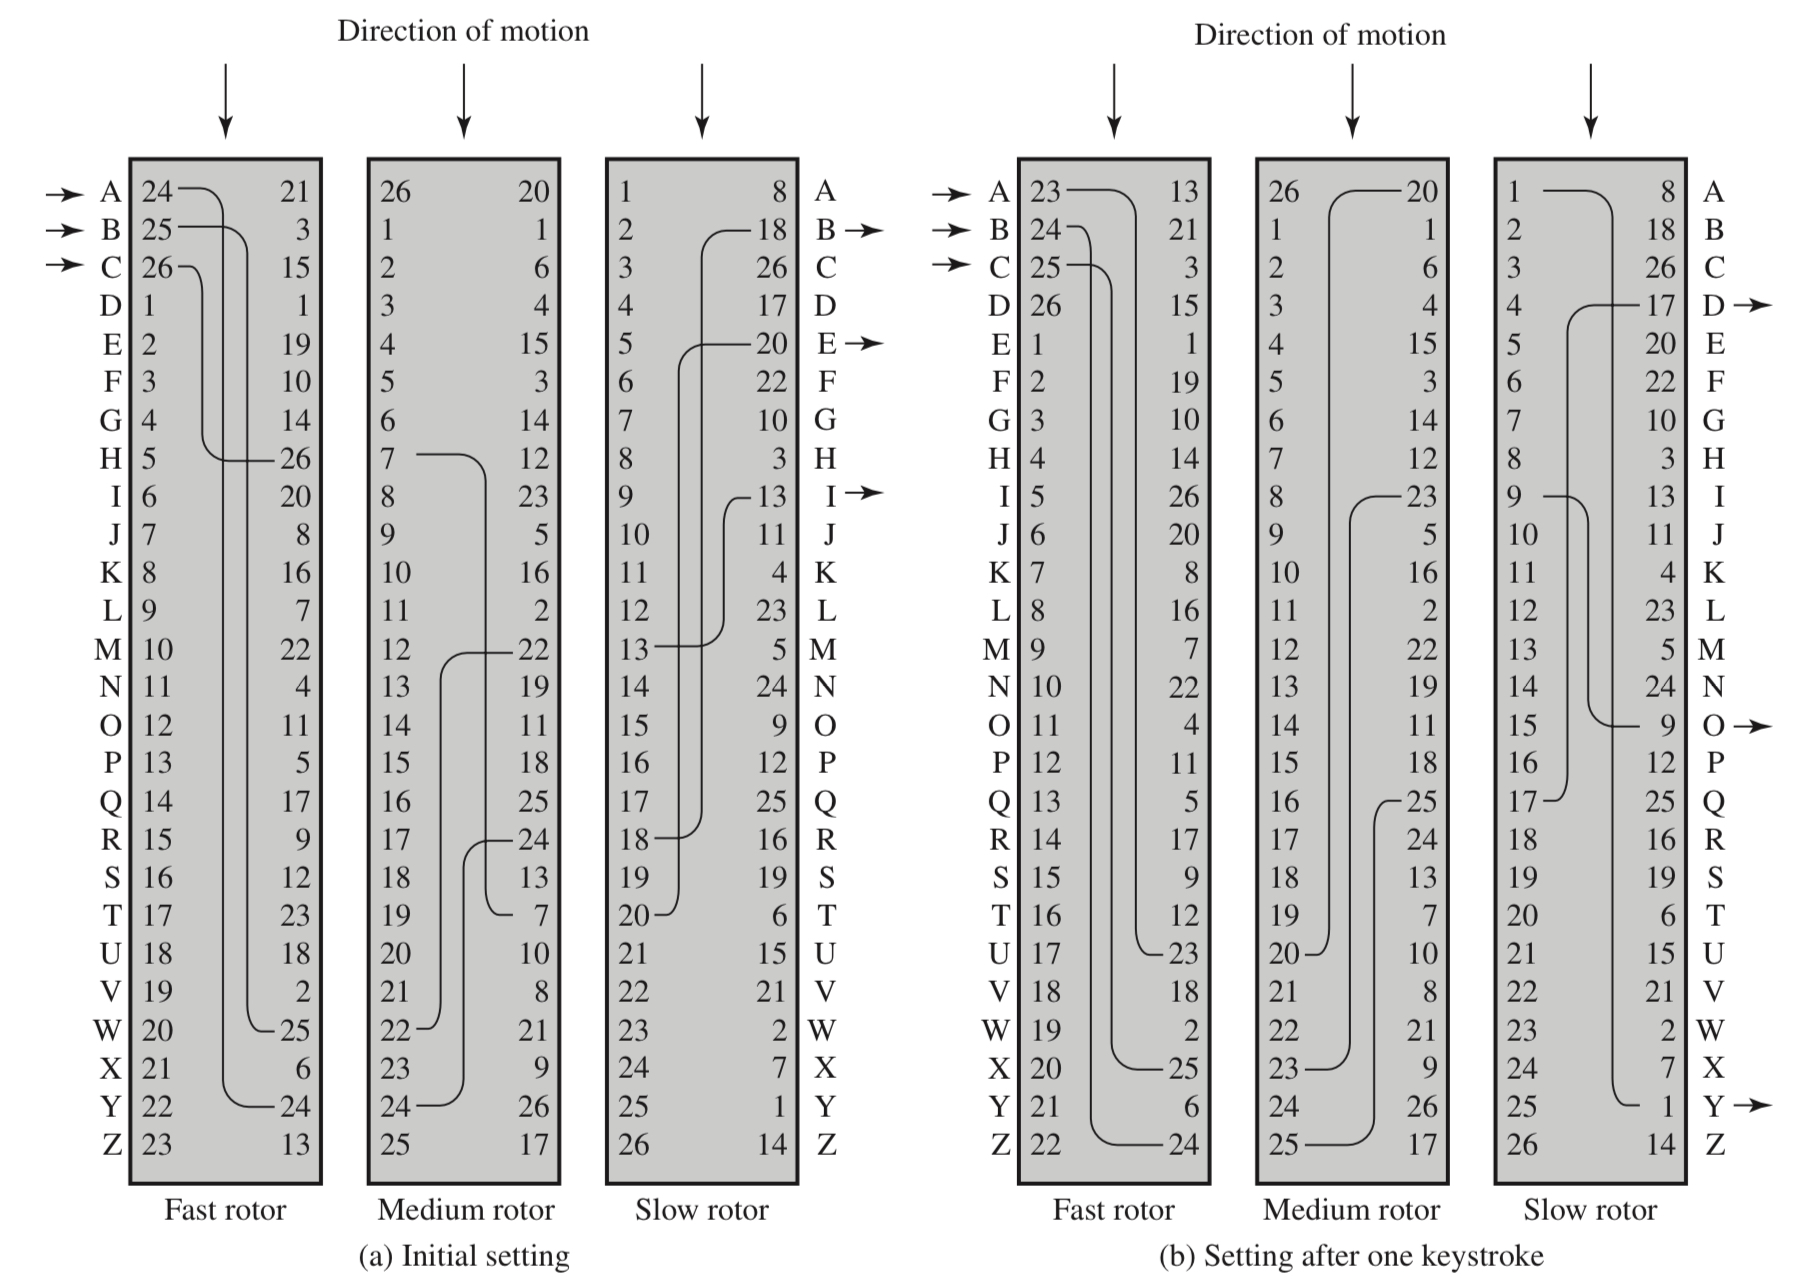
\includegraphics[width=0.8\textwidth]{img/Concatenazione_crittosistemi.png}
    \caption{Macchina a rotori}
\end{figure}

\subsubsection{Enigma}
La macchina Enigma è una macchina elettromeccanica portatile utilizzata per cifrare e decifrare
messaggi segreti. È stata utilizzata in Germania durante la seconda guerra mondiale.
La decodifica dei messaggi è molto complessa, vista la grande quantità di combinazioni possibili.

Se ho a una macchina che per essere decifrata ha bisogno di un tempo più alto della validità 
dei dati, allora posso dire che è sicura.

Il modo per decodificare i messaggi è stato fondamentale sapere che il messaggio iniziava con
una parola chiave, che era sempre la stessa. Sapendo questo, si poteva decodificare il messaggio
riducendo notevolmente l'insieme delle chiavi disponibili per la decodifica.
Conoscevano quindi il \textbf{plaintext}.

La concatenzione di crittosistemi è molto sicura, ma non è sicura contro gli attacchi
dove si conosce il plaintext.

\section{Classificazione dei livelli di sicurezza}
La classificazione si basa sulla difficoltà di violare il sistema, quindi sul tipo di 
attacchi a cui resiste.
\begin{itemize}
    \item \textbf{Known Cipher Text Attack}: l'attaccante conosce il testo cifrato.
    \item \textbf{Known Plaintext Attack}: l'attaccante vede il testo in chiaro e il corrispondente testo cifrato.
    \item \textbf{Chosen Plaintext Attack}: l'attaccante sceglie il testo in chiaro e conosce il corrispondente testo cifrato.
    \item \textbf{Adaptive Chosen Ciphertext Attack}: l'attaccante può continuamente scegliere il testo in chiaro e vedere il corrispondente testo cifrato.
\end{itemize}
La classifica è in base alla potenza che gli do nell'attaccarmi.
L'obiettivo è costruire un sistema che sia sicuro contro 
gli attacchi Adaptive Chosen Ciphertext Attack.
\section{Cifrari a flusso e a blocchi}
Un \textbf{cifrario a flusso} crittografa un flusso di dati digitali un bit
o un byte alla volta. Esempi di cifrari a flusso classici sono il
cifrario di Vigenère con autochiave e il cifrario di Vernam. Nell'ideale,
si utilizzerebbe una versione del cifrario di Vernam con one-time pad, in
cui lo stream di chiavi ha la stessa lunghezza dello stream di bit in chiaro.
Tuttavia, perché questo sia praticamente realizzabile, lo stream di chiavi deve
essere fornito in anticipo ad entrambi gli utenti attraverso un canale indipendente
e sicuro, il che può rappresentare una sfida logistica se il traffico dati
previsto è di grandi dimensioni.

Di conseguenza, per ragioni pratiche, il generatore di stream di bit deve
essere implementato come una procedura algoritmica, in modo che lo stream di
bit crittografico possa essere prodotto da entrambi gli utenti. In questo
approccio, il generatore di stream di bit è un algoritmo controllato dalla chiave
e deve produrre uno stream di bit crittograficamente robusto. I due utenti devono
condividere solo la chiave di generazione, e ognuno può generare lo stream di chiavi.

Un \textbf{cifrario a blocchi} tratta un blocco di testo in chiaro come un'entità
unica e produce un blocco di testo cifrato della stessa lunghezza. Di solito,
si utilizza una dimensione di blocco di $64$ o $128$ bit. Allo stesso modo del 
cifrario a flusso, i due utenti condividono una chiave di crittografia simmetrica.
Utilizzando alcune delle modalità di funzionamento spiegate in precedenza, un
cifrario a blocchi può essere usato per ottenere lo stesso effetto di un cifrario
a flusso.

Molto più sforzo è stato dedicato all'analisi dei cifrari a blocchi, poiché
sembrano essere applicabili a una gamma più ampia di applicazioni rispetto ai
cifrari a flusso. La maggior parte delle applicazioni crittografiche simmetriche
basate su rete fa uso di cifrari a blocchi. Pertanto, le discussioni in questo
contesto si concentreranno principalmente su di essi.

\subsection{Electronic Code Book}
Il ``Electronic Code Book" (\verb|ECB|) è una
delle modalità di funzionamento di un cifrario a blocchi, utilizzato per
crittografare un blocco di testo di lunghezza fissa. In questa modalità,
ogni blocco di testo in chiaro viene crittografato separatamente utilizzando
la stessa chiave. Non c'è alcuna dipendenza tra i blocchi di testo in chiaro
durante il processo di crittografia. Pertanto, gli stessi blocchi di testo in
chiaro generano gli stessi blocchi di testo cifrato. Tuttavia, questo comporta
il rischio di sicurezza in quanto pattern di testo in chiaro simili generano
pattern di testo cifrato simili, rendendo il sistema vulnerabile a un'analisi
statistica. Nonostante questa debolezza, l'\verb|ECB| è ancora utilizzato in alcuni
scenari in cui la semplicità e la velocità sono prioritarie rispetto alla
sicurezza, come per la crittografia di dati non sensibili o per applicazioni
specifiche in cui la perdita di alcuni blocchi non compromette la sicurezza
complessiva del sistema.

La modalità più semplice è la modalità di codifica elettronica (\verb|ECB|), in cui
il testo in chiaro viene gestito un blocco alla volta e ogni blocco di testo
in chiaro viene crittografato utilizzando la stessa chiave. Il termine ``codice"
è utilizzato perché, per una data chiave, esiste un testo cifrato univoco per
ogni blocco di testo in chiaro di b bit. Pertanto, possiamo immaginare un'enorme
tabella di corrispondenza in cui vi è una voce per ogni possibile modello
di testo in chiaro di $b$ bit che mostra il relativo testo cifrato corrispondente.
\begin{figure}[H]
    \centering
    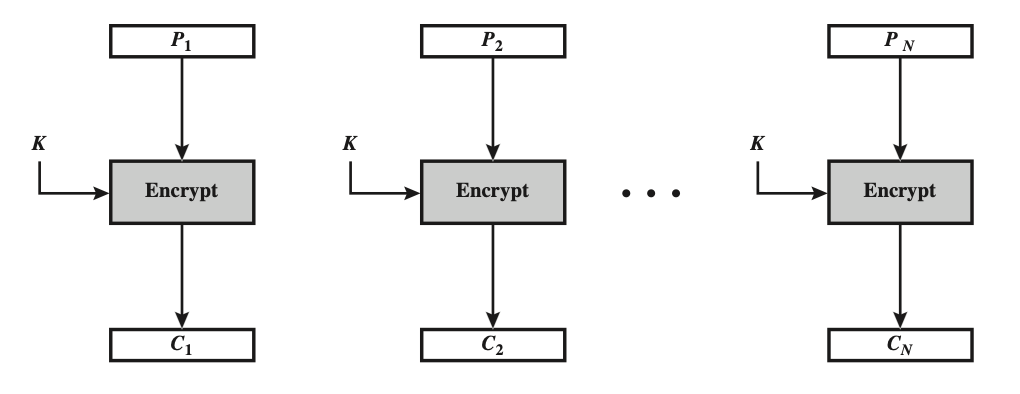
\includegraphics[width=0.5\textwidth]{img/electriccodeblock.png}
    \caption{Electronic Code Book}
\end{figure}

\subsection{Cipher Block Chaining}

La modalità di funzionamento ``Cipher Block Chaining'' (\verb|CBC|) è un metodo
di crittografia a blocchi che introduce un certo grado di indipendenza tra i
blocchi di testo in chiaro durante il processo di crittografia. Funziona come
segue:

\begin{enumerate}
    \item Prima di crittografare, viene generato un vettore di inizializzazione
    casuale noto come vettore di inizializzazione (\texttt{IV}). Questo vettore
    è combinato con il primo blocco di testo in chiaro tramite un'operazione di
    \texttt{XOR}.
    
    \item Il risultato di questa operazione \texttt{XOR} viene quindi
    crittografato utilizzando l'algoritmo di cifratura a blocchi insieme
    alla chiave.
    
    \item Il blocco di testo cifrato risultante viene poi combinato con il
    blocco di testo successivo prima della crittografia. Questo collegamento
    tra i blocchi di testo in chiaro aiuta a rompere la correlazione tra i
    blocchi di testo in chiaro, migliorando la sicurezza rispetto alla modalità
    di Electronic Code Book (\texttt{ECB}).
    
    \item Questo processo continua per tutti i blocchi di testo in chiaro
    successivi, garantendo che ciascun blocco di testo cifrato dipenda dal
    blocco di testo in chiaro precedente, oltre che dalla chiave.
\end{enumerate}

La decodifica avviene seguendo lo stesso processo in ordine inverso,
utilizzando il vettore di inizializzazione e la chiave per ottenere il
testo in chiaro originale.

La modalità \texttt{CBC} è considerata più sicura dell'\texttt{ECB} poiché
introduce una
dipendenza tra i blocchi di testo in chiaro, rendendo più complessa l'analisi
statistica e aumentando la resistenza agli attacchi crittoanalitici.
Tuttavia, è importante gestire correttamente il vettore di inizializzazione
per garantire la sicurezza e l'integrità del sistema di crittografia.
\[ C_j = E(K, [C_{j-1} \oplus P_j]) \]
\begin{figure}[H]
    \centering
    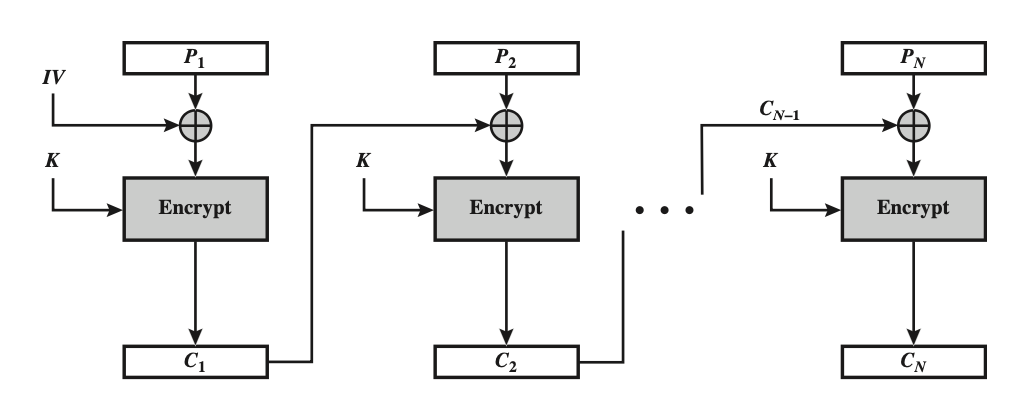
\includegraphics[width=0.8\textwidth]{img/CBC.png}
    \caption{Cipher Block Chaining}
\end{figure}
\subsection{Cipher Feedback}
Per \verb|AES|, \verb|DES| o qualsiasi altro cifrario a blocchi, la crittografia viene eseguita
su un blocco di \(b\) bit. Nel caso di \verb|DES|, \(b = 64\), e nel caso di \verb|AES|,
\(b = 128\). Tuttavia, è possibile convertire un cifrario a blocchi in un cifrario
a flusso utilizzando una delle modalità di funzionamento: la modalità di
Feedback di Cifratura (\verb|CFB|) e la modalità di Feedback di Output (\verb|OFB|).

Un cifrario a flusso elimina la necessità di aggiungere padding a un messaggio
per renderlo un numero intero di blocchi. Inoltre, può funzionare in tempo reale.
Pertanto, se viene trasmesso uno stream di caratteri, ogni carattere può essere
cifrato e trasmesso immediatamente utilizzando un cifrario a flusso orientato
ai caratteri.

Una proprietà desiderabile di un cifrario a flusso è che il testo cifrato abbia
la stessa lunghezza del testo in chiaro. Pertanto, se vengono trasmessi caratteri
di $8$ bit, ogni carattere dovrebbe essere cifrato per produrre un output di
testo cifrato di $8$ bit. Se vengono prodotti più di $8$ bit, la capacità di
trasmissione viene sprecata.

La modalità \verb|CFB| è illustrata nello schema. In questa modalità, il testo in chiaro
è diviso in segmenti di \(s\) bit, dove \(s\) è la dimensione dell'unità di
trasmissione. Durante la crittografia, viene utilizzato un registro a scorrimento
di \(b\) bit inizializzato con un vettore di inizializzazione (\verb|IV|). I
primi \(s\) bit più significativi dell'output della funzione di crittografia
vengono combinati con il primo segmento di testo in chiaro \(P_1\) tramite
l'operazione \texttt{XOR} per produrre l'unità di testo cifrato \(C_1\), che viene quindi
trasmessa. Il contenuto del registro a scorrimento viene spostato a sinistra di
\(s\) bit e \(C_1\) viene inserito nei \(s\) bit meno significativi del registro
a scorrimento. Questo processo continua fino a quando tutti i segmenti di testo
in chiaro sono stati crittografati.

Per la decodifica, viene utilizzato lo stesso schema, ad eccezione che l'unità
di testo cifrato ricevuta viene combinata tramite \verb|XOR| con l'output della funzione
di crittografia per produrre l'unità di testo in chiaro. È importante notare che
viene utilizzata la funzione di crittografia e non quella di decodifica. Questo
è facilmente spiegabile. Sia \(\texttt{MSBs}(X)\) definita come i \(s\) bit più significativi
di \(X\). Quindi

\[ C_1 = P_1 \oplus \texttt{MSBs}[E(K, IV)] \]

Di conseguenza, riarrangiando i termini:

\[ P_1 = C_1 \oplus \texttt{MSBs}[E(K, IV)] \]
\begin{figure}[H]
    \centering
    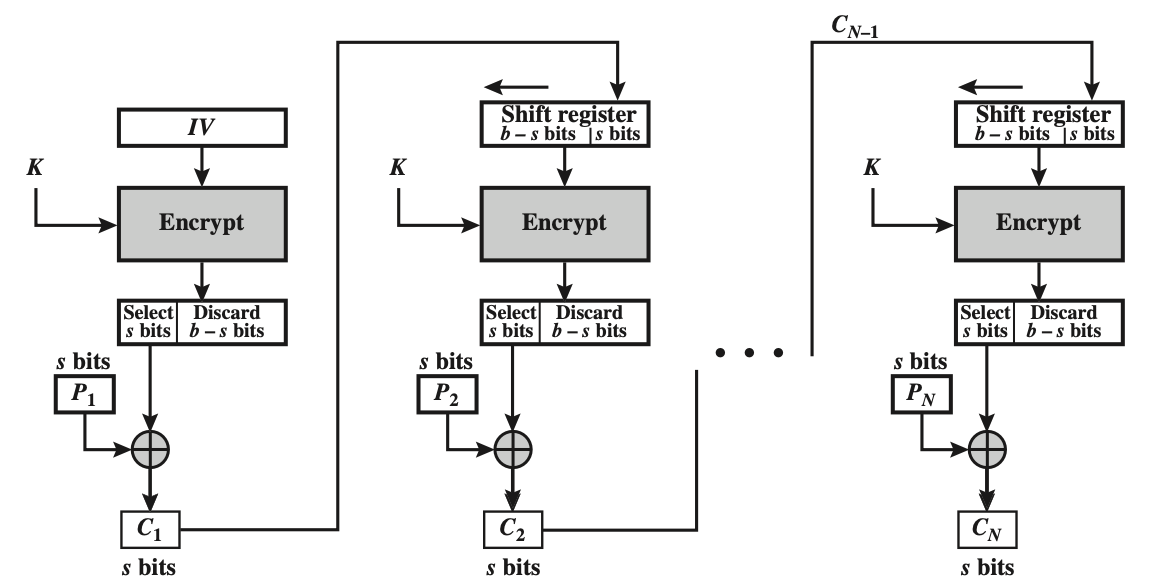
\includegraphics[width=0.8\textwidth]{img/cipherFeedback.png}
    \caption{Cipher Feedback}
\end{figure}
\subsection{Output Feedback}
La modalità di Feedback di Output (\verb|OFB|) ha una struttura simile a
quella di \verb|CFB|. Per \verb|OFB|, l'output della funzione di crittografia viene
retroalimentato e diventa l'input per crittografare il blocco successivo
di testo in chiaro. In \verb|CFB|, l'output dell'unità \verb|XOR| viene
retroalimentato e diventa l'input per crittografare il blocco successivo.
L'altra differenza è che la modalità \verb|OFB| opera su blocchi completi
di testo
in chiaro e testo cifrato, mentre \verb|CFB| opera su un sottoinsieme di \(s\) bit.
La crittografia \verb|OFB| può essere espressa come:

\[ C_j = P_j \oplus E(K, O_{j-1}) \]
\[ O_{j-1} = E(K, O_{j-2}) \]

Un po' di riflessione dovrebbe convincerti che possiamo riscrivere
l'espressione di crittografia come:

\[ C_j = P_j \oplus E(K, [C_{j-1} \oplus P_{j-1}]) \]

Riarrangiando i termini, possiamo dimostrare che la decodifica funziona:

\[ P_j = C_j \oplus E(K, [C_{j-1} \oplus P_{j-1}]) \]

\begin{figure}[H]
    \centering
    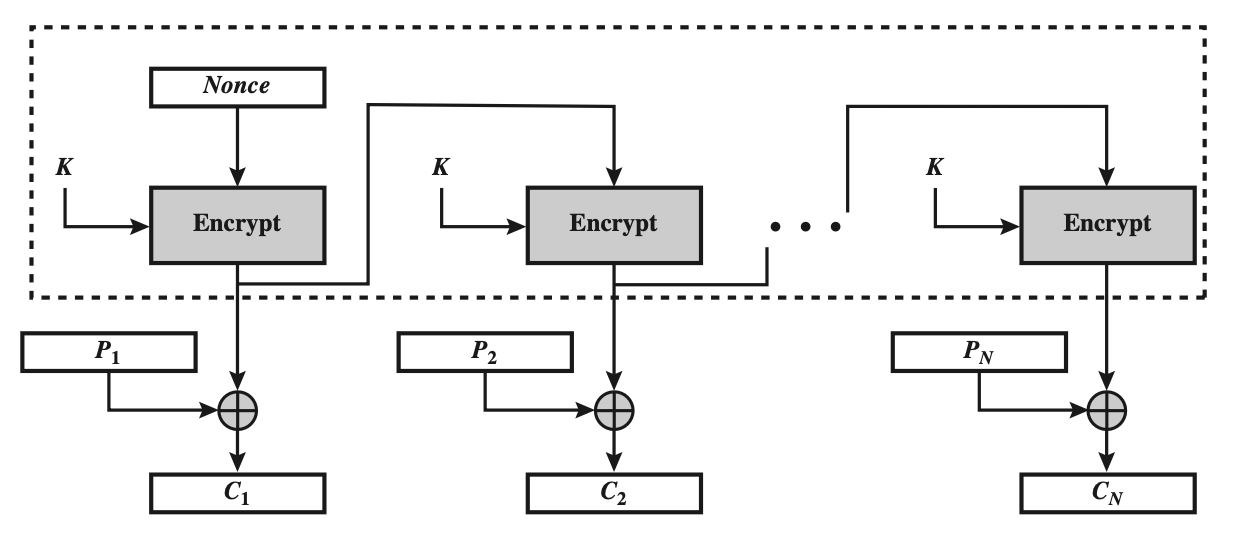
\includegraphics[width=0.8\textwidth]{img/outputFeedback.png}
    \caption{Output Feedback}
    \label{fig:outputFeedback}
\end{figure}
I blocchi di output della cifratura, \(O_i\), dipendono solo dalla chiave
e dal vettore di inizializzazione (\verb|IV|) e non dipendono dal testo
in chiaro. Pertanto, per una data chiave e \verb|IV|, lo stream di bit di
output utilizzato per l'operazione \texttt{XOR} con lo stream di bit in chiaro è fisso.
Se due messaggi diversi avessero un blocco identico di testo in chiaro
nella stessa posizione, un attaccante sarebbe in grado di determinare
quella parte dello stream \(O_i\).

Un vantaggio del metodo \verb|OFB| è che gli errori di bit nella trasmissione non
si propagano. Ad esempio, se si verifica un errore di bit in \(C_1\), solo
il valore ripristinato di \(P_1\) viene influenzato; i blocchi di testo in
chiaro successivi non vengono corrotti. Con \verb|CFB|, \(C_1\) serve anche come
input al registro a scorrimento e quindi causa corruzioni aggiuntive a valle.

Lo svantaggio di \verb|OFB| è che è più vulnerabile a un attacco di modifica dello
stream di messaggi rispetto a \verb|CFB|. Considera che complementare un bit nel
testo cifrato complementa il bit corrispondente nel testo in chiaro
ripristinato. Pertanto, possono essere effettuate modifiche controllate
al testo in chiaro ripristinato. Questo potrebbe rendere possibile per un
avversario, apportando le modifiche necessarie alla parte di checksum del
messaggio e alla parte di dati, modificare il testo cifrato in modo che non
sia rilevato da un codice di correzione degli errori.

\verb|OFB| ha la struttura di un tipico cifrario a flusso, poiché il cifrario
genera uno stream di bit come funzione di un valore iniziale e di una chiave,
e questo stream di bit viene operato con \verb|XOR| con i bit del testo in chiaro.
Lo stream generato che viene operato con \verb|XOR| con il testo in chiaro è
indipendente dal testo in chiaro stesso; questo è evidenziato da riquadri
tratteggiati in Figura (\ref{fig:outputFeedback}). Una differenza rispetto
ai cifrari a flusso è che \verb|OFB| crittografa il testo in chiaro un blocco
intero alla volta, dove tipicamente un blocco è di $64$ o $128$ bit. Molti
cifrari a flusso crittografano un byte alla volta.

\section{Rete di Feistel}
Moltissimi algoritmo di cifratura a blocchi utilizzano tale struttura.
La struttura di Feistel è una struttura di rete iterativa che è stata
progettata per essere utilizzata in cifrari a blocchi.
Tale struttura ha delle caratteristiche distintive:
\begin{itemize}
    \item L'input viene diviso in due metà.
    \item Esegue molteplici \textit{round} di cifratura, dove in ogni round 
    le due metà vengono elaborate in modo come segue:
    \begin{itemize}
        \item La metà sinistra diventa la metà destra del round precedente.
        \[
          L_i = R_{i-1}  
        \]
        \item La metà destra diventa l'applicazione della funzione di \texttt{XOR}
        tra la metà sinistra del round precedente e l'output della funzione $f$ che prende 
        in input la metà destra del round precedente e la chiave del round precedente.
        \[
            R_i = L_{i-1} \oplus f(R_{i-1}, K_{i-1})
        \]
    \end{itemize}
    \item La struttura è simmetrica, il che significa che la decodifica 
    avviene semplicemente invertendo l'ordine delle chiavi usate per la cifratura.
    \begin{itemize}
        \item \[ R_{i-1} = L_i \]
        \item \[L_{i-1} = R_i \oplus f(L_i, K_i)\]
    \end{itemize}
\end{itemize}
Il vantaggio è che le funzioni $f$ usate sono \textbf{one-way}.
\begin{tcolorbox}[title=One-way function]
    Una funzione $f: \{0,1\}^* \rightarrow \{0,1\}^*$ è \textbf{one-way} se esiste un algoritmo 
    che in tempo polinomiale mappa $x$ in $f(x)$ per ogni $x \in \{0,1\}^*$ e per ogni algoritmo 
    probabilistico polinomiale $\mathcal{A}$, ogni polinomio $p(\cdot)$
    e ogni intero $n$ sufficientemente grande, si ha che la probabilità che $\mathcal{A}$
    trovi un $x$ tale che $f(\mathcal{A}(f(x))) = f(x)$ è minore di $1/p(n)$.
\end{tcolorbox}
Anche se un algoritmo ha accesso a un metodo efficiente per generare valori che, una volta
processati dalla funzione $f$, producono un output, è estremamente improbabile che tale algoritmo 
possa invertire la funzione e trovare l'input originale dato l'output, almeno senza una 
quantità impraticabile di tempo e risorse.
\begin{figure}[H]
    \centering
    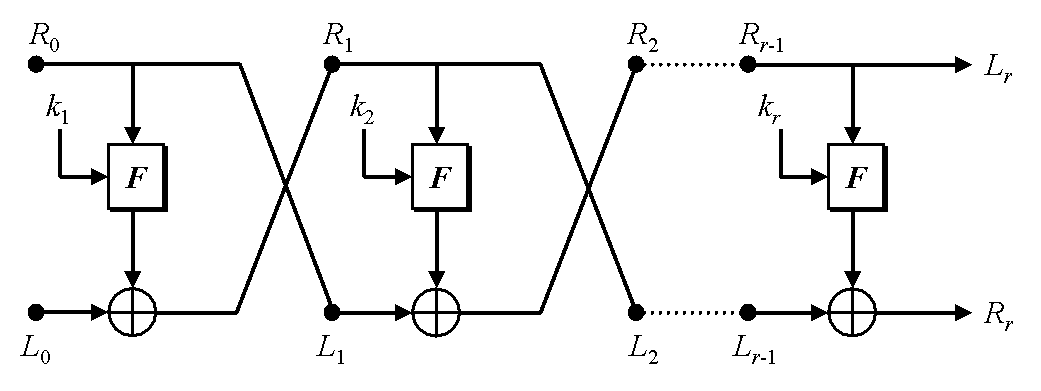
\includegraphics[width=0.8\textwidth]{img/feistel.png}
    \caption{Rete di Feistel}
\end{figure}
\section{Data Encryption Standard - \texttt{DES}}
\texttt{DES} è un cifrario a blocchi a chiave simmetrica che utilizza una struttura di Feistel.

La chiave è di $56$ bit, ma in realtà sono $64$ bit, di cui $8$ sono di parità, ed 
opera su blocchi di $64$ bit. 
L'algoritmo esegue una permutazione iniziale dei bit del blocco di testo in chiaro,
nota come \textit{Initial Permutation (IP)}, che riordina i bit secondo uno schema
fisso predefinito. Questo è seguito da 16 round di cifratura che consistono in espansione,
mescolamento con una chiave di round derivata dalla chiave principale, sostituzione tramite S-Box
e una permutazione finale. La funzione di round prende input dalla metà destra del blocco di dati
e la chiave di round, producendo un output che è poi combinato con la metà sinistra attraverso
un'operazione XOR.

Dopo l'ultimo round, le due metà del blocco vengono scambiate, e questo è seguito da una
\textit{Final Permutation (FP)}, che è l'inverso della permutazione iniziale. Il risultato
è il blocco di testo cifrato. La decodifica con \texttt{DES} segue lo stesso processo ma
in ordine inverso, utilizzando le chiavi di round in ordine inverso.

Nonostante la sua ampiamente testata sicurezza, la principale vulnerabilità di \texttt{DES}
risiede nella lunghezza della chiave. Tecniche come l'attacco a forza bruta, che era
teoricamente possibile ma non praticabile al tempo della sua creazione, sono divenute
fattibili con l'avanzamento della potenza di calcolo. Per questo motivo, \texttt{DES}
è stato sostituito da \texttt{AES} come standard approvato dal NIST (\textit{National
Institute of Standards and Technology}) per la cifratura di informazioni sensibili.
\subsection{Funzione di round}
La funzione di round prende in input $32$ bit e una chiave di round di $48$ bit e produce
un output di $32$ bit. La funzione di round è composta da quattro passaggi:
\begin{enumerate}
    \item \textbf{Espansione}: i $32$ bit di input vengono espansi a $48$ bit tramite una
    permutazione fissa.
    \item \textbf{Mescolamento}: i $48$ bit vengono combinati con la chiave di round tramite
    un'operazione di \texttt{XOR}.
    \item \textbf{Sostituzione}: Dopo il mescolamento con la chiave di round, i $48$ bit vengono
    passano attraverso $8$ \texttt{S-BOX}, ciascuno dei quali sostituisce $6$ bit con $4$ bit. 
    Sono lineari e complesse per aggiungere sicurezza alla cifratura.
    \item \textbf{Permutazione}: i $32$ bit vengono permutati tramite una permutazione fissa.
\end{enumerate}
L'alternanza di sostituzioni mediante \texttt{S-BOX}, permutazioni mediante permutazioni fisse
e espansioni forniscono la \textbf{confusione} e la \textbf{diffusione}, concetti introdotti
da \texttt{Shannon} e che sono alla base di molti cifrari moderni.

\begin{tcolorbox}[title=Confusione]
    Si tratta della relazione tra il testo in chiaro e la chiave. Deve essere difficile
    dedurre la chiave a partire dal testo cifrato. Ogni bit del testo cifrato deve
    dipendere da molti bit della chiave.
\end{tcolorbox}

\begin{tcolorbox}[title=Diffusione]
    Si tratta della capacità di un algoritmo di distribuire le correlazioni statistiche
    del testo lungo tutto l'alfabeto utilizzato dall'algoritmo di cifratura, rendendo quanto 
    più difficile un attacco statistico.
\end{tcolorbox}
\chapter{Teoria dei numeri}
\section{Proprietà dei numeri}

La teoria dei numeri è una branca fondamentale della matematica che studia le proprietà degli interi e delle loro relazioni. Nel contesto della teoria dei numeri, diversi concetti chiave emergono dall'analisi delle operazioni e degli insiemi numerici.

\begin{tcolorbox}[title={Operazioni chiuse}]
Un'operazione si dice chiusa se l'operazione applicata a due numeri naturali restituisce un numero naturale.
\[
  \mathbb{N} \, \texttt{op} \, \mathbb{N} \to \mathbb{N}  
\]
Ad esempio, l'addizione e la moltiplicazione sono operazioni chiuse sugli interi.
\end{tcolorbox}

Quando un'operazione non è chiusa? La divisione, non produce sempre un numero naturale. Gli insiemi sono inoltre caratterizzati da proprietà che li rendono unici.

\begin{tcolorbox}[title={Proprietà commutativa}]
  \[
    a \, \texttt{op} \, b = b \, \texttt{op} \, a
  \]
L'addizione e la moltiplicazione sono esempi di operazioni che soddisfano la proprietà commutativa.
\end{tcolorbox}

\begin{tcolorbox}[title={Proprietà associativa}]
  \[
    \forall a, b, c \in A \qquad a \, \texttt{op} \, (b \, \texttt{op} \, c) = (a \, \texttt{op} \, b) \, \texttt{op} \, c
  \]
La proprietà associativa è verificata dall'addizione e dalla moltiplicazione su diversi insiemi numerici.
\end{tcolorbox}

\begin{tcolorbox}[title={Elemento neutro}]
  \[
    a \, \texttt{op} \, e = a
  \]
  quindi 
  \[
    \exists e \in A \texttt{ t.c. }\forall a \in A \, a \, \texttt{op} \, e = e \, \texttt{op} \, a = a
  \]
L'elemento neutro per l'addizione è lo zero, mentre per la moltiplicazione è l'unità.
\end{tcolorbox}

\begin{tcolorbox}[title={Elemento inverso}]
  \[
    \forall a \in A \, \exists a^{-1} \in A \texttt{ t.c. } a \, \texttt{op} \, a^{-1} = a^{-1} \, \texttt{op} \, a = e
  \]
Alcuni esempi di elementi inversi includono l'opposto di un numero per l'addizione e il reciproco di un numero non nullo per la moltiplicazione.
\end{tcolorbox}

Ogni volta che definiamo delle strutture matematiche che soddisfano tali proprietà, si parla di gruppi. Un \textbf{gruppo} è
una struttura algebrica che rispetta determinate regole, tra cui chiusura, associatività, presenza di un elemento neutro e di un elemento inverso.

Prendiamo in considerazione i numeri naturali rispetto all'operazione di somma. Hanno l'inverso? No, quindi non è un gruppo. Tuttavia,
se aggiungessimo altri elementi e arrivassimo ai numeri interi, allora avremmo un gruppo rispetto alla somma. Allo stesso modo, se
considerassimo i numeri interi rispetto alla moltiplicazione (\textit{senza lo zero}), non avremmo l'inverso. In questo caso, dovremmo aggiungere
gli inversi e arrivare ai numeri razionali, che costituiscono un gruppo rispetto alla moltiplicazione.

Capita spesso di avere strutture che non sono gruppi. In questi casi, si possono seguire due approcci: ridurre la struttura eliminando
gli elementi che non soddisfano le proprietà del gruppo o espandere la struttura aggiungendo elementi in modo da soddisfare tali proprietà.

Vorremmo lavorare su un'algebra diversa, possibilmente con gruppi finiti. In particolare, ci concentreremo su gruppi che costituiscono
l'algebra alla base dei nostri algoritmi crittografici. Utilizzeremo funzioni che sono facili da calcolare ma difficili da invertire,
comunemente conosciute come \textbf{one-way function}. Queste funzioni si basano sull'algebra moltiplicativa.

Successivamente, esamineremo anche la crittografia ellittica, che si basa su un'algebra diversa, operando su curve ellittiche. Tuttavia,
gli algoritmi fondamentali rimarranno gli stessi, utilizzando però un'algebra additiva.

\section{Classe di equivalenza $\mathbb{Z}_n$}
Possiamo dire che:
\[
  \mathbb{Z}_n \equiv \mathbb{Z}_n \qquad a \equiv b \pmod{n} \iff (a \mod n) = (b \mod n)
\]
Quindi due numeri sono equivalenti se hanno lo stesso resto nella divisione per $n$.
Ad esempio, $5 \equiv 11 \pmod{3}$, perché entrambi hanno resto 2 nella divisione per 3.

Quando abbiamo una relazione di equivalenza possiamo costruire l'insieme degli oggetti equivalenti tra loro. 
L'insieme degli insiemi di oggetti equivalenti forma una \textbf{partizione}, gli elementi di tale 
partizione sono detti \textbf{classi di equivalenza} e si denotano mediante parentesi quadre di un elemento di tale classe.
Ogni singola classe di equivalenza può essere rappresentata da un qualsiasi elemento della classe stessa. 
\[
  \mathbb{Z}_n = \{0,1,2,3,\dots, n-1\}
\]

Un'analogia può essere fatta con le ore. Se sono le 10:00, allora sono anche le 22:00,
perché entrambe sono equivalenti a 10:00 $\pmod{12}$, o con le frazioni. È l'insieme 
delle classi di equivalenza tra numeri naturali dove due coppie sono 
equivalenti se hanno lo stesso prodotto incrociato, quindi il prodotto 
dei medi è uguale al prodotto degli estremi. Ad esempio, $2 \times 3 = 1 \times 6$. 
\[
  \frac{1}{2} \equiv \frac{3}{6}
\]
La rappresentazione canonica di una classe di equivalenza in $\mathbb{Z}_n$ è il suo
rappresentante minimo, ovvero un numero naturale compreso tra 0 e $n-1$.

Su tale insieme voglio definire delle operazioni.
\subsection{Somma}
La somma di due classi di equivalenza è definita come la classe di
equivalenza della somma dei rappresentanti. Ad esempio, se voglio
calcolare $[2] + [3]$, allora calcolo $2 + 3 = 5$ e la classe di equivalenza
di 5 è $[5]$. In generale, la somma di due classi di equivalenza è la classe
di equivalenza della somma dei rappresentanti.
\[
  [a] + [b] \stackrel{\Delta}{=} [a + b]
\]
Tale rappresentazione è buona solo se il risultato è indipendente dagli elementi 
delle due classi originali.
\subsubsection{Proprietà}
\begin{itemize}
  \item \textbf{Commutativa}: $\forall a, b \,[a] + [b] = [b] + [a]$.
  \item \textbf{Associativa}: $\forall a, b, c \,[a] + ([b] + [c]) = ([a] + [b]) + [c]$.
  \item \textbf{Elemento neutro}: $\exists e \in \mathbb{Z}_n \, \forall a \, [a] + [a] = [a] + [a] = [a]\qquad e = 0$.
  \item \textbf{Elemento inverso}: $\forall a \, \exists a^{-1} \in \mathbb{Z}_n \,
  \text{t.c.} \, [a] + [a^{-1}] = [a^{-1}] + [a] = [e] \qquad a^{-1} = -a$.
\end{itemize}
L'insieme $\mathbb{Z}_n$ con l'operazione di somma forma un \textbf{gruppo abeliano}, (
\textit{abeliano} perché commutativo).
\subsection{Moltiplicazione}
La moltiplicazione di due classi di equivalenza è definita come la classe di
equivalenza del prodotto dei rappresentanti. Ad esempio, se voglio
calcolare $[2] \cdot [3]$, allora calcolo $2 \cdot 3 = 6$ e la classe di equivalenza
di 6 è $[6]$. In generale, la moltiplicazione di due classi di equivalenza è la classe
di equivalenza del prodotto dei rappresentanti.
\[
  [a] \cdot [b] \stackrel{\Delta}{=} [a \cdot b]
\]
Tale rappresentazione è buona solo se il risultato è indipendente dagli elementi
delle due classi originali.
\subsubsection{Proprietà}
\begin{itemize}
  \item \textbf{Commutativa}: $\forall a, b \,[a] \cdot [b] = [b] \cdot [a]$.
  \item \textbf{Associativa}: $\forall a, b, c \,[a] \cdot ([b] \cdot [c]) = ([a] \cdot [b]) \cdot [c]$.
  \item \textbf{Elemento neutro}: $\exists e \in \mathbb{Z}_n \, \forall a \, [a] \cdot [a] = [a] \cdot [a] = [a]\qquad e = 1$.
\end{itemize}
L'insieme $\mathbb{Z}_n$ con l'operazione di moltiplicazione forma un \textbf{semigruppo}, 
ovvero un gruppo senza l'elemento inverso.
Per ottenere un gruppo, devo aggiungere l'elemento inverso. Per ottenere tale elemento,
quindi passare da un semigruppo ad un gruppo, 
posso seguire diverse strade; arricchire l'insieme con nuovi elementi, oppure
eliminare elementi.

Consideriamo l'insieme $\mathbb{Z}_n - \{0\}$ con l'operazione di moltiplicazione e consideriamo 
un esempio con $n = 15$.
\[
  \mathbb{Z}_{15} - \{0\} = \{1,2,3,4,5,6,7,8,9,10,11,12,13,14\}
\]
\begin{itemize}
  \item L'inverso moltiplicativo di $1$ è $1$.
  \item L'inverso moltiplicativo di $2$ è $8$ ($2 \cdot 8 = 16 \equiv 1 \pmod{15}$).
  \item L'inverso moltiplicativo di $3$ non c'è.
  \item \dots
\end{itemize}
Notiamo che non tutti gli elementi hanno un inverso moltiplicativo, quindi non 
posso costruire un gruppo. Per ottenere un gruppo, devo eliminare gli elementi
che non hanno un inverso moltiplicativo.
L'insieme $\mathbb{Z}_{15} - \{0, 3, 5, 6, 9, 10, 12\}$ che sarà quindi:
\[
  \mathbb{Z}_{15}^* = \{1,2,4,7,8,11,13,14\}
\]
Abbiamo quindi definito l'insieme $\mathbb{Z}_n^*$:
\[
  \mathbb{Z}_n^* = \{a \in \mathbb{Z}_n \, | \, \texttt{mcd}(a, n) = 1\}
\]
Ovvero l'insieme dei numeri che sono relativi primi con $n$.
Moltiplicando due numeri relativamente primi con $n$, ottengo un numero
relativamente primo con $n$. L'operazione di moltiplicazione è chiusa in $\mathbb{Z}_n^*$.
\begin{theorem}[Teorema di Eulero]
  Per ogni $a, b \, \exists x,y \, ax + by = \texttt{mcd}(a,b)$
\end{theorem}
Se $a \in \mathbb{Z}_n^*$ allora $\texttt{mcd}(a, n) = 1$ per definizione e quindi
\[
  ax + ny = 1
\] 
\[
  ax = 1 - ny
\]
\[
  ax \equiv 1 \pmod{n}
\]
Quindi la classe di equivalenza di $x$ è l'inverso moltiplicativo di $a$.
La necessità di lavorare con gruppi nasce dal fatto che in informatica
è necessario lavorare con insiemi finiti, in questo caso algebre su insiemi 
finiti, in particolare sui gruppi, in modo da manipolare gli elementi in 
base alle proprietà.
\section{Gruppi e generatori}
Sia $\mathcal{G}$ un gruppo, un operatore $\otimes$. Sia $g$ un elemento di $\mathcal{G}$.
\[
  g = g^1 \qquad g \otimes g = g^2 \qquad g \otimes g \otimes g = g^3 \qquad \dots \qquad g \otimes g 
  \otimes g \otimes \dots \otimes g = g^n
\]
Continuando a moltiplicare $g$ per se stesso, non arriverò ad un qualsiasi $n$ generico, poiché 
il gruppo è finito. Quindi, supponiamo  che arrivi a $g \otimes g 
\otimes g \otimes \dots \otimes g = g^{\lvert \mathcal{G} \rvert}$ e che l'esponente successivo 
sia $g^{\lvert \mathcal{G} \rvert + 1}$. Per il \textbf{pumping lemma} avrò sicuramente 
almeno un elemento ripetuto.
\begin{theorem}
  Per ogni gruppo $\mathcal{G}$ finito, per ogni $a \in \mathcal{G}$, 
  \[
    a^{\lvert \mathcal{G} \rvert} = 1
  \]
\end{theorem}
Da questo teorema segue che se sicuramente $a^{\lvert \mathcal{G} \rvert} = 1$ ovvero l'elemento neutro,
ma per un gruppo $\mathcal{G}$ finito, potrei avere anche che per un qualche
$a^i = 1$.

Se prendo tutte le potenze di $g$ ottengo un sottogruppo dell'insieme $\mathcal{G}$, un sottogruppo 
continua ad essere un gruppo. Se quello che ottengo è un sottogruppo proprio, ovvero 
un sottogruppo che non è tutto l'insieme $\mathcal{G}$, allora $G$ è ciclico e $g$ è un 
\textbf{generatore} di $\mathcal{G}$.
\begin{theorem}
  Sia $\mathcal{G}'$ è sottogruppo di $\mathcal{G}$, allora $\lvert \mathcal{G}' \rvert \mid
  \lvert \mathcal{G} \rvert$.
\end{theorem}
\subsubsection{Esempio}
\[
  \mathbb{Z}_{15}^* = \{1,2,4,7,8,11,13,14\}
\]
\begin{itemize}
  \item $1$
  \item $2 \cdot 2 = 4 \cdot 2 = 8 \cdot 2 = 16$ quindi $2^4 \equiv 1 \pmod{15}$
  \item $4 \cdot 4 = 16 \equiv 1 \pmod{15}$
  \item $7 \cdot 7 = 49 \equiv 4, 4 \cdot 7 = 28 \equiv 13, 13 \cdot 7 = 91 \equiv 1 \pmod{15}$
  \item $8 \cdot 8 = 64 \equiv 4, 4 \cdot 8 = 32 \equiv 2, 2 \cdot 8 = 16 \equiv 1 \pmod{15}$
  \item $11 \cdot 11 = 121 \equiv 1 \pmod{15}$
  \item $13 \cdot 13 = 169 \equiv 4, 4 \cdot 13 = 52 \equiv 7, 7 \cdot 13 = 91 \equiv 1 \pmod{15}$
  \item $14 \cdot 14 = 196 \equiv 1 \pmod{15}$
\end{itemize}
La cardinalità di $\mathbb{Z}_{15}^*$ è $8$, ma questo gruppo non è ciclico, poiché non esiste un
elemento generatore che generi tutto il gruppo.
\subsection{Generatori primi}
Se prendo $\mathbb{Z}_{n}^*$ con $n$ primo, allora $\mathbb{Z}_{n}^*$ è ciclico, poiché
ogni elemento di $\mathbb{Z}_{n}^*$ è un generatore di $\mathbb{Z}_{n}^*$.
In generale un numero primo non può essere scomposto in fattori, quindi:
\[
  \mathbb{Z}_{p}^* = \{1,2,3,\dots,p-1\}
\]
\subsubsection{Esempio}
\[
  \mathbb{Z}_{7}^* = \{1,2,3,4,5,6\}
\]
\begin{itemize}
  \item $1$
  \item $2 \cdot 2 = 4 \cdot 2 = 8 \equiv 1 \pmod{7}$
  \item $3 \cdot 3 = 9 \equiv 2, 2 \cdot 3 = 6, 6 \cdot 3 = 18 \equiv 4, 4 \cdot 3 = 12 \equiv 5, 5 \cdot 3 = 15 \equiv 1 \pmod{7}$
  \item $4 \cdot 4 = 16 \equiv 2, 2 \cdot 4 = 8 \equiv 1 \pmod{7}$
  \item $5 \cdot 5 = 25 \equiv 4, 4 \cdot 5 = 20 \equiv 6, 6 \cdot 5 = 30 \equiv 2, 2 \cdot 5 = 10 \equiv 3, 3 \cdot 5 = 15 \equiv 1 \pmod{7}$
  \item $6 \cdot 6 = 36 \equiv 1 \pmod{7}$
\end{itemize}
Abbiamo che $\mathbb{Z}_{7}^*$ è ciclico, poiché esiste un generatore che genera tutto il gruppo, in questo 
caso $3$ e $5$.

\subsection{Probabilità dei numeri primi}
\begin{theorem}[Densità dei numeri primi]
  La densità dei numeri primi è proporzionale al numero di bit che compongono il numero.
\end{theorem}
Suppongo di avere un numero casuale $n$ di $k$ bit, allora la probabilità che $n$ sia primo è 
$\frac{1}{k}$. Supponiamo di voler comporre un numero $n$ di $k$ bit, utilizzo un algoritmo
che mi generi tale numero. 

Per verificare che tale numero sia primo, utilizzo una algoritmo casuale 
che sceglie casualmente un numero $a$ tra $1$ e $n-1$ e verifica che il numero 
scelto sia primo. Statisticamente circa la metà dei numeri scelti sono testimoni del fatto 
che un numero non sia primo. Se il test fallisce e mi dice che il numero non è primo, allora
termino. Se il test ha esito positivo allora scelgo un altro numero $a$ e ripeto il test di 
primalità.
Se tutte le volte che scelgo un numero $a$ il test ha esito positivo, allora la probabilità 
di accettare la primalità di $n$ è $\frac{1}{2^t}$, dove $t$ è il numero di volte che ho
ripetuto il test (\textit{eventi indipendenti}), abbassando la probabilità di errore notevolmente.

Sulla base di questo ragionamento, siamo in grado di generare numeri primi molto grandi.
\chapter{Crittografia a chiave pubblica}
\section{Crittografia a chiave pubblica}
L'idea di crittografia a chiave pubblica è quella di avere due chiavi, una
pubblica $P_k$ e una privata $S_k$. La chiave pubblica è nota a tutti, mentre
quella privata è nota solo al proprietario. 
Con codifica avviene con la chiave pubblica, mentre la decodifica avviene con la
chiave privata.

Ovviamente l'idea di fondo è avendo in mano il testo cifrato non si riesce a
risalire al testo in chiaro senza la chiave privata. Chiunque può cifrare un
messaggio, ma solo il proprietario della chiave privata può decifrarlo.

In un sistema a chiave pubblica abbiamo i seguenti algoritmi:
\begin{itemize}
    \item Un algoritmo di generazione delle chiavi:
    \[
        \mathcal{G}: 1^k \to (P_k, S_k) 
    \]
    Dove $1^k$ è un parametro che indica la lunghezza della chiave, ovvero il \textit{security parameter}.
    \item Un algoritmo di encription:
      \[
        \mathcal{E}: m, P_k \to \mathcal{E}(m, P_k)
    \]
    \item Un algoritmo di decription:
    \[
          \mathcal{D}: C, S_k \to D(C, P_k)
    \]
\end{itemize}
Ovviamente vale la seguente relazione:
\begin{equation}
    \forall m \quad \mathcal{D}(\mathcal{E}(m, P_k), S_k) = m
\end{equation}
Oltre al fatto che decriptare un messaggio a partire dal testo cifrato senza 
la chiave privata è computazionalmente intrattabile. L'idea è che più la chiave
è lunga più è difficile rompere il sistema. L'idea è che il security parameter
$k$ è proporzionale alla lunghezza della chiave e al crescere di $k$ cresce
la sicurezza del sistema.

Gli algoritmi citati sono algoritmi probabilistici polinomiali. Se voglio 
affermare che tali algoritmi sono polinomiali l'input che rappresenta la 
lunghezza della chiave non può essere 
rappresentato in binario, perché la lunghezza della chiave sarebbe
esponenziale nel numero di bit utilizzati per rappresentare il numero. 
Sulle macchine di Turing la dimensione del problema è data dal numero di 
celle del nastro di input. Utilizzando la teoria della complessità 
basata su tali macchine, o in ogni caso su sistemi dove la dimensione 
dell'input è lo spazio che occupa nella nostra rappresentazione. Per 
voler dire che un algoritmo è polinomiale nel \textbf{valore del 
security parameter} e non nel modo in cui è rappresentato, imponiamo 
che il security parameter sia rappresentato in \textbf{unario}, ovvero 
tanti uni quanti la lunghezza della chiave.

\section{Diffie-Hellman}
Il problema di Diffie-Hellman è il seguente: Alice e Bob vogliono
scambiarsi un segreto senza che Eve lo possa intercettare. Lo strumento 
utilizzato per risolvere il problema è del logaritmo discreto.

Si fissa a priori un numero primo $p$ e un generatore $g$ di $\mathbb{Z}_p^*$.
Un agente A sceglie un numero $x \in_R \{1, \dots, p-1\}$ e calcola $g^x \mod p$. 
Un agente B sceglie un numero $y \in_R \{1, \dots, p-1\}$ e calcola $g^y \mod p$.

\begin{figure}[H]
    \centering
    \begin{tabular}[H]{l|l|l}
        & \textbf{Public} & \textbf{Private} \\
        \hline
        A & $g^x \mod p$ & $x$ \\
        \hline
        B & $g^y \mod p$ & $y$ \\
    \end{tabular}
\end{figure}

A questo punto A e B possono calcolare $g^{xy} \mod p$ e $g^{yx} \mod p$, che coincidono.

Il sistema è sicuro perché calcolare $g^{xy} \mod p$ è computazionalmente intrattabile. Avendo 
a disposizione $g^x$ e $g^y$ non è possibile calcolare $g^{xy}$. Se sappiamo rispondere al problema 
del logaritmo discreto, allora possiamo risolvere il problema di Diffie-Hellman, tale algoritmo 
potrebbe esistere, ma non è stato ancora trovato.

Sia $\mathcal{A} \in \texttt{PPT}$ che calcola $g^{xy} \mod p$ a partire da $g^x \mod p$ e $g^y \mod p$. 
Usiamo $\mathcal{A}$ per costruire un algoritmo $\mathcal{B}$ che risolve il problema del logaritmo discreto,
ma tale dimostrazione non è ancora stata data, perciò non l'algoritmo di Diffie-Hellman non è dimostrabilmente 
sicuro. non siamo in grado di dire che rompere Diffie-Hellman è almeno difficile quanto risolvere il problema
del logaritmo discreto.

\subsection{Ipotesi di Diffie-Hellman}
Qualcuno potrebbe costruire un algoritmo che si basa sull'ipotesi che l'algoritmo di Diffie-Hellman sia sicuro.
\begin{tcolorbox}[title = Ipotesi di Diffie-Hellman]
    Siano $x, y, z$ dei numeri causali scelti in $\{1, \dots, p-1\}$, allora è difficile 
    distinguere ($g^x, g^y, g^{xy}$) da ($g^x, g^y, g^z$).
\end{tcolorbox}

Il concetto di distinguibilità è un concetto probabilistico, ovvero che la possibilità di poter 
distinguere due insiemi di elementi è trascurabile. Ovvero che la probabilità di distinguere 
sia inferiore a $1/2 + \epsilon$, dove $\epsilon$ è trascurabile. Quindi l'attaccante non abbia 
alcun vantaggio rispetto ad un attaccante che non ha alcuna informazione.
Se un attaccante avesse anche un minimo vantaggio, allora potrebbe utilizzare tale vantaggio per
ottenere informazioni sul segreto. Tale vantaggio può essere utilizzato per ottenere l'informazione 
totale mediante esperimenti ripetuti.

\section{Rivest Shamir Adleman - RSA}
$g^x$ è una funzione che è facile da calcolare, ma è difficile da invertire, ovvero calcolare $x$
a partire da $g^x$. Una funzione con questa proprietà è detta \textbf{one-way function}. Il protocollo di 
Diffie-Hellman è sicuro se e solo se esiste una one-way function.
Vorremmo che la one-way function sia anche \textbf{trapdoor}, ovvero che esista un algoritmo 
efficiente che permetta di invertire la funzione. Tale algoritmo è detto \textbf{trapdoor algorithm}.
La trapdoor è una informazione aggiuntiva che permette di invertire la funzione.

Siano $p, q$ due numeri primi molto grandi, $n = pq$. Sia $e$ un numero casuale tale che 
\texttt{mcd}(e, $\varphi(n)$) = 1, dove $\varphi(n) = (p-1)(q-1)$, ovvero il numero di Eulero. Scegliamo 
une elemento $d$ co-primo con $\varphi(n)$ tale che $de \equiv 1 \mod \varphi(n)$.
La chiave pubblica è la coppia $(n, e)$, mentre la chiave privata è la coppia $(n, d)$.
\subsubsection{Algoritmo di cifratura}
\[
  \mathcal{E}: m, (n, e) \mapsto m^e \mod n  
\]
\subsubsection{Algoritmo di decifratura}
\[
  \mathcal{D}: c, (n, d) \mapsto c^d \mod n
\]
\subsection{Funzionamento}
Proviamo a prendere un messaggio $m$ e a cifrarlo con la chiave pubblica $(n, e)$,
e proviamo a decodificarlo con la chiave privata $(n, d)$.
\[
  (m^e)^d = m^{ed} = m^{k\varphi(n) + 1} = m \cdot (m^{\varphi(n)})^k \equiv m \mod n  
\]
Infatti $d\cdot e$ è congruo a 1 modulo $\varphi(n)$, quindi $d\cdot e = k\varphi(n) + 1$.
Per il teorema del resto cinese, $m^{k\varphi(n) + 1} \equiv m$, e non solo per gli elementi 
di $\mathbb{Z}_n^*$.

La funzione one way è la funzione di codifica, quindi $m^e$, l'inversa di 
$m^e$ è la radice $e$-esima, ovvero $m = c^{1/e}$, ma per calcolare la radice $e$-esima
ad oggi non esiste un algoritmo efficiente. L'unico modo per calcolare la radice $e$-esima
è calcolare $d$ e decifrare il messaggio, quindi $d$ è l'informazione trapdoor.

Ci piacerebbe dimostrare che se fossimo in grado di invertire la radice 
e-esima di un numero allora saremmo in grado di fattorizzare $n$, o di calcolare 
il residuo quadratico. Se fosse vero, allora RSA sarebbe sicuro, ma non è stato ancora
dimostrato ad oggi. L'unica sicurezza di RSA è l'esistenza dell'ipotesi di RSA.
\subsection{Attacchi a RSA}
Ci sono casi in cui RSA è stato attaccato, il motivo però era legato alla cattiva 
implementazione dell'algoritmo, e non all'algoritmo in sé.
Quando parliamo di un crittosistema in realtà parliamo di un insieme di algoritmi,
e non di un singolo algoritmo. L'algoritmo di generazione delle chiave impone 
la scelta \textbf{casuale} di $e$ in modo uniforme con gli elementi 
primi con $\varphi(n)$, ma se non fosse casuale, allora potremmo avere dei problemi.
\subsubsection{Attacco sulla base di messaggi piccoli}
Inoltre, in caso di messaggi piccoli, quindi se $m^e < n$, vuol dire che 
non applico nemmeno l'operazione di modulo, e vuol dire in particolare che 
la radice $e$-esima di $m^e$ è una normale radice $e$-esima nell'aritmetica 
dei numeri interi, e quindi è facile da calcolare.
Lavorando con messaggi che a livello numerico sono piccoli, allora 
invertiamo tutto facilmente, più è piccola $e$, più è facile avere 
messaggi che elevati a $e$ sono più piccoli di $n$. Bisogna quindi
star attenti a scenari in cui $m^e < n$.
\subsubsection{Attacco sulla base di messaggi sparsi}
Altri problemi che potrebbe avere RSA sono legati allo spargimento dei 
messaggi.
Immaginiamo di avere un messaggio:

\begin{center}
  \texttt{Buongiorno, il suo voto è 30L}\\
  \texttt{Buongiorno, il suo voto è 30}\\
  \texttt{Buongiorno, il suo voto è 29}\\
  \dots\\
  \texttt{Buongiorno, il suo voto è 0}\\
\end{center}
Uno che vuole decifrare il messaggio può prendere i $32$ messaggi e
cifrarli tutti, per poi distinguerli.
Se con RSA devo codificare messaggi che sono presi da un insieme piccolo,
devo far attenzione perché potrei venir attaccato da qualcuno che utilizza 
la stessa chiave pubblica.
\subsubsection{Attacco sulla informazione parziale}
Siamo sicuri che tutti i bit di questa inversa siano difficili da calcolare?
Non è che sulla radice $e$-esima di $m^e$ ci sono dei bit che sono più facili 
da calcolare? Ai fini di dire che il sistema è sicuro, non è 
sufficiente dire che il cypertext non si sappia ricavare il plaintext,
vorremmo dire che dal cypertext non si riesca a ricavare nessuna informazione 
binaria sul plaintext. Ma come possiamo definire tale proprietà?
\subsubsection{Attacco sulla base di messaggi ripetuti}
Per difendersi da tale problema, aggiungo un po' di rumore al messaggio,
ovvero aggiungo un po' di bit casuali al messaggio, in modo tale che con 
alta probabilità il messaggio non sia mai uguale. In questo modo, anche se
il messaggio è sempre lo stesso, il cypertext è sempre diverso, utilizzando 
quindi la probabilistic encryption.
\section{Sicurezza di un crittosistema}
RSA è sicuro perché non conosciamo un algoritmo probabilistico polinomiale 
per calcolare la radice $e$-esima di un numero. Ma cosa vuol dire?
Se esistesse un algoritmo probabilistico polinomiale per calcolare la radice 
$e$-esima di un numero con probabilità $\frac{1}{k}$, sarebbe un problema,
perché reiterando l'algoritmo $k$ volte, avrei una probabilità di successo.

Se fossimo nello scenario in cui con un $a\in_R \mathbb{Z}_n^*$, l'algoritmo 
mi dia risposta corretta con probabilità $\frac{1}{k}$, potremmo dichiararci 
tranquilli? No, perché potrebbero attaccare sempre.

Fissando $a$ e scegliendo $r \in_R \mathbb{Z}_n^*$, calcolo $(a\cdot r)^e \mod n$,
se prendo un elemento casuale di $\mathbb{Z}_n^*$ e lo elevo ad $e$, ottengo
l'oggetto che è distribuito uniformemente in $\mathbb{Z}_n^*$. Sappiamo che
l'elevamento di $r$ alla $e$-esima è distribuito uniformemente in $\mathbb{Z}_n^*$, 
perché $e$ è stata scelta in maniera tale che la radice $e$-esima dia esattamente 
$r$. Quindi $r^e$ è una funzione invertibile, di conseguenza la funzione che mappa $r$ in 
$r^e$ è una funzione biettiva, quindi un elemento scelto uniformemente in $\mathbb{Z}_n^*$
viene mappato da $r^e$ in un elemento scelto uniformemente scelto in $\mathbb{Z}_n^*$.
Ogni volta che prendiamo un elemento e creiamo una suriezione dello stesso insieme, 
se l'elemento di partenza è scelto uniformemente, il risultato della suriezione, che nella 
sostanza è una permutazione, è scelto uniformemente.

Se prendiamo $r^e$ e lo moltiplichiamo per $a$, otteniamo un elemento che è distribuito
uniformemente in $\mathbb{Z}_n^*$, perché $a$ è scelto uniformemente in $\mathbb{Z}_n^*$, 
poiché la moltiplicazione per $a$ è una funzione biettiva, perché $a$ ammette inverso.

Siamo partiti da un elemento fissato e abbiamo costruito un elemento distribuito uniformemente
e causale, se a quell'elemento applichiamo l'algoritmo della radice $e$-esima, otteniamo
$\frac{1}{k}$ di probabilità di successo, ma se ripetiamo l'algoritmo $k$ volte, abbiamo
una probabilità di successo di $1$, rendendo quindi l'algoritmo indipendente dalla $a$ di 
partenza.
\[
  ar^e \rightarrow \sqrt[e]{ar^e} = r \sqrt[e]{a}
\]
Quindi se prendo il risultato e lo divido per $r$, ottengo $\sqrt[e]{a}$,
che è distribuito uniformemente in $\mathbb{Z}_n^*$, perché $r$ è distribuito uniformemente.

Ed ecco che abbiamo un algoritmo che a partire da una blackbox che con $a$ causale 
calcola correttamente la radice $e$-esima di $a$ una volta su $k$, abbiamo una macchina 
che con $a$ fissato calcola la radice $e$-esima di $a$ con probabilità $1$.

La macchina che calcola la radice $e$-esima di $a$ darà una sequenza di bit, che
potrebbe essere la radice $e$-esima di $a$, oppure no. Bisognerebbe riconoscere la risposta
corretta, rielevando il risultato ad $e$, se ottengo l'input allora la risposta è 
corretta, altrimenti no.

Quindi abbiamo trasformato un algoritmo che funziona una volta su $k$ in un algoritmo
che funziona in un tempo medio di $k$.
\begin{tcolorbox}[title=Definizione di sicurezza]
  Diciamo che un sistema è attaccabile se il tempo medio per attaccarlo è polinomiale.
\end{tcolorbox}
Se esistesse un qualsiasi algoritmo in grado di attaccare la radice $e$-esima di $a$,
con una probabilità polinomiale in $k$, riusciamo a costruire un algoritmo che calcola
la stessa cosa con un tempo medio polinomiale in $k$.

Visto che partiamo  dall'idea che non esista un algoritmo probabilistico polinomiale 
in grado di calcolare la radice $e$-esima di $a$, allora non esiste un algoritmo
che sia in grado di calcolarlo con una probabilità che sia polinomialmente piccola.
Quindi la \textbf{probabilità di successo è più piccola di qualsiasi polinomio}, dove per polinomio 
si intende:
\[
  \probP[\texttt{attacco}] < \frac{1}{k}\quad \forall c
\]
Fissando un polinomio, con chiavi corte, però, la possibilità di trovare un polinomio esiste, 
perciò bisogna correggere tale definizione.
\begin{equation}
  \forall c \exists \bar{k} \forall k > \bar{k}\quad\probP[\texttt{attacco}] < k^{-c}
\end{equation}
Per attacco non intendiamo solo il fatto di non poter essere in grado di poter calcolare la 
radice $e$-esima di $a$, ma anche il fatto di non essere in grado di capire 
\textbf{informazioni binarie}.

L'algoritmo che calcola la radice $e$-esima di $a$ è l'algoritmo che calcola la
la fattorizzazione di $n$, la fattorizzazione di $n$ è l'informazione 
binaria che vogliamo proteggere.textbf{trapdoor} che permette di risolvere 
il problema.
\begin{tcolorbox}[title=Fattorizzazione di $n$]
  Si pensa che non esista un algoritmo \texttt{PPT} che dati $n$, $e$ e $a$,
  calcola $\sqrt[e]{a} \in \mathbb{Z}_n^*$ con probabilità polinomiale.
\end{tcolorbox}
\subsection{Utilizzo pratico di RSA}
Nel caso pratico il costo computazionale di RSA è molto alto, infatti codificare 
un blocco di $k$ bit con RSA richiede $k$ esponenziazioni modulari, ovvero $k^3$, 
un costo computazionale molto alto. Per questo motivo RSA viene utilizzato per
codificare una chiave di sessione, che viene utilizzata per codificare
il messaggio con un algoritmo simmetrico, che è molto più veloce di RSA.
Tipicamente l'algoritmo utilizzato è l'algoritmo simmetrico \texttt{AES} (\ref{section:des}).

Tra l'altro vi è una notevole differenza con Diffie-Hellman, infatti in Diffie-Hellman
riesco a scambiarmi un'unica chiave, a meno che non faccia un nuovo scambio di chiavi,
ogni volta.

Se si parte dall'idea che la crittografia simmetrica sia meno sicura della crittografia
asimmetrica, allora si può pensare di utilizzare una chiave di sessione diversa dopo 
un certo periodo. Con RSA è possibile fare questo, perché è possibile scambiarsi
chiavi diverse, mentre con Diffie-Hellman non è possibile, perché si dovrebbero scambiare
chiavi diverse ogni volta, e questo è molto costoso. La generazione della chiave di sessione 
per Diffie-Hellman è molto costosa, per via delle Certification Authority, che devono
essere coinvolte nel processo di generazione della chiave di sessione per certificare 
le chiavi pubbliche.

\section{Crittosistema di Micali per la codifica di un singolo bit}
\subsubsection{Algoritmo di generazione delle chiavi}
Si sceglie un numero primo $p_1$ e un numero $p_2$ tale che moltiplicati tra loro
diano un numero $n$ tale che $n = p_1p_2$. I due numeri devono essere scelti in modo
casuale con $\frac{k}{2}$ bit ciascuno, dove $k$ è la lunghezza della chiave. Sia 
$y \in_R$ ai non quadrati con simbolo di Jacobi $1$ modulo $n$. Ricordiamo che per 
costruire un numero non quadrato causale con simbolo di Jacobi $1$ basta scegliere un numero
casuale e verificare che il simbolo di Jacobi sia $1$, ovvero che appartenga 
a $\mathbb{Z}_n^*$, se non lo è si sceglie un altro
numero casuale e si ripete il procedimento. A questo punto verifico che il simbolo 
di Legendre rispetto a $p_1$ e $q_1$ sia $-1$. 

La chiave pubblica è:
\[
  P_k = (n, y)
\]
La chiave privata è:
\[
  S_k = (p_1, p_2)
\]
L'ipotesi di base è che sia difficile fattorizzare $n$, ma il problema di 
riferimento sarà il problema del residuo quadratico, ovvero il problema di
calcolare la radice quadrata di un numero modulo $n$.
\subsubsection{Algoritmo di codifica}
L'algoritmo di codifica prende un bit $b$, sia $x \in_R \mathbb{Z}_n^*$, se 
$b$ è $0$ allora $c = x^2 \mod n$, altrimenti $c = xy^2 \mod n$. 
$x^2$ è un quadrato casuale di $\mathbb{Z}_n^*$, mentre $xy^2$ è un 
non quadrato con simbolo di Jacobi $1$. Se prendo un quadrato con simbolo di 
Jacobi $1$ e lo moltiplico per un non quadrato con simbolo di Jacobi $1$ ottengo
un non quadrato con simbolo di Jacobi $1$. Se il quadrato è casuale, allora 
ottengo un non quadrato casuale con simbolo di Jacobi $1$ distribuito uniformemente
tra tutti i non quadrati con simbolo di Jacobi $1$.

Il risultato è che la codifica di $0$ è un quadrato a caso, mentre la codifica di $1$ è
un non quadrato a caso con simbolo di Jacobi $1$.
\[
  \mathcal{E}: \{0, 1\} \to x \in_R \mathbb{Z}_n^*
\]
\[
  f(x) = \begin{cases}
    x^2 \mod n & \text{se } b = 0\\
    xy^2 \mod n & \text{se } b = 1
  \end{cases}
\]
\subsubsection{Algoritmo di decodifica}
L'algoritmo di verifica prende in input $c$ e verifica se $c$ è un quadrato 
rispetto a $p_1$ e $p_2$, ovvero se $c$ è un residuo quadratico modulo $p_1$ e
modulo $p_2$. Se $c$ è un quadrato rispetto a $p_1$ e $p_2$ allora $b = 0$,
se entrambe le verifiche falliscono allora $b = 1$, in altri casi non siamo in presenza 
di un cypertext valido.
\[
  \left(\frac{c}{p_1}\right) = \left(\frac{c}{p_2}\right) = 1 \qquad \text{allora } b = 0
\]
\[
  \left(\frac{c}{p_1}\right) = \left(\frac{c}{p_2}\right) = -1 \qquad \text{allora } b = 1
\]
\subsection{Rompere il crittosistema di Micali}
Rompere tale protocollo significherebbe disporre di un algoritmo $\mathcal{A}$ che preso in 
input in cyphertext $c$ e la chiave pubblica $P_k$ restituisce $b$ con probabilità
diversa da $\frac{1}{2}$, poiché siamo in un contesto binario.

Un attaccante quindi dovrebbe essere in grado di ottenere un vantaggio rispetto 
a qualcuno che non conosce nulla, ovvero che indovini con probabilità $\frac{1}{2}$.
Il vantaggio consiste nell'allontanarsi da $\frac{1}{2}$, sia in positivo che in negativo, 
poiché se si allontana in negativo basta invertire il risultato per ottenere
un vantaggio positivo.

Il numero di esperimenti deve essere tale che la differenza delle probabilità sia
maggiore di $\frac{1}{2}$, ma il numero di esperimenti deve essere un numero 
polinomiale, in modo tale da poter osservare tali esperimenti in tempo polinomiale.
\begin{tcolorbox}[title = Sicurezza]
  \begin{equation}
    \forall c \, \exists \bar{k} \, \forall k \geq \bar{k} \quad \mid \probP[\texttt{Successo}] - \frac{1}{2} \mid  > k^{-c}
  \end{equation}
\end{tcolorbox}
Supponiamo che la probabilità di successo sia maggiore di $\frac{1}{2} + \epsilon$ e vorrei che la probabilità di successo sia quindi 
prossima a $1$. Per farlo eseguo due tipologie di esperimenti, il primo ripete l'esperimento $k$ volte e mediante l'algoritmo che 
ha a disposizione il vantaggio è $\frac{1}{2} + \epsilon$, mentre il secondo esperimento ripete l'esperimento $k$ volte e mediante
esperimenti casuali, ovvero senza l'algoritmo, ottiene un vantaggio di $\frac{1}{2}$. Ripetendo l'esperimento un numero abbastanza grande di 
volte si ottiene il risultato desiderato, poiché basterebbe visualizzare le due distribuzioni per vedere in cosa differiscono. L'algoritmo 
quindi indovina con probabilità $1$. Più $\epsilon$ è piccolo, più esperimenti sono necessari per ottenere il risultato desiderato. 
Servirebbe quindi stimare, dato un $\epsilon$ fissato, il numero di esperimenti necessari per ottenere il risultato desiderato.
\subsubsection{Limite di Chernoff} \label{limite_chernoff}
\begin{tcolorbox}[title = Limite di Chernoff]
  Siano $X_1, \dots, X_n$ variabili casuali e binarie indipendenti con probabilità 
  di successo $\probP[X_i = 1] > \frac{1}{2}$ e $\probP[X_i = 0] = 1 - \probP[X_i = 1]$.
  La probabilità che più della metà delle variabili casuali siano $1$ è:
  \[
    \mathcal{P} = \sum_{i = \frac{n}{2} + 1}^n \binom{n}{i} \probP[X_i = 1]^i \probP[X_i = 0]^{n - i}
  \]
  \[
    \mathcal{P} \geq 1 - e^{-2n\left(p - \frac{1}{2}\right)^2}
  \]
  Tale formula dice che la probabilità che più della metà degli eventi dia $1$ è 
  esponenzialmente vicina a $1$, dove l'eponenzialmente è in funzione di $n$.
  \[
    \probP[\texttt{errore}] = e^{-2 \epsilon n}
  \]
  Dove $\epsilon$ è il vantaggio.
\end{tcolorbox}
Supponiamo di volere $e^{-2 \epsilon n} < \frac{1}{2^k}$, quindi:
\[
  e^{-2c\epsilon^2 n} < 2^{-k}
\]
\[
  -2\epsilon^2 n < c' - k 
\]
\[
  n > \frac{c' - k}{2\epsilon^2}
\]
Se $\epsilon$ è polinomiale in $k$ allora $n$ è polinomiale in $k$.
Di conseguenza, se il vantaggio è polinomiale in qualche security parameter, allora
si riesce ad ottenere una quantità di errore nel security parameter che è
esponenzialmente piccola, scegliendo una quantità di esperimenti polinomiale in esso.

Un sistema è attaccato nel momento in cui esiste un algoritmo polinomiale in 
grado di romperlo.

Nel momento in cui $\epsilon$ è un $k^{-c}$, allora $n$ (\textit{dove $n$ è il numero di
esperimenti}) è polinomiale in $k$.

Visto che l'ipotesi di partenza è che non esistano algoritmi probabilistici polinomiali in grado
di rompere il sistema (\textit{vero}) e visto che abbiamo dimostrato che esiste tale algoritmo (\textit{falso}), allora
l'algoritmo di Micali è sicuro.
\subsubsection{Costruzione degli esperimenti indipendenti}

Una volta capito che la costruzione di $n$ esperimenti indipendenti funziona, bisogna 
capire come costruirli. Supponiamo che la probabilità di successo sia $\frac{1}{2} + \epsilon$ e
di disporre di un algoritmo $\mathcal{A}$ che prende in input un numero $z$ 
con $\left(\frac{z}{n}\right) = 1$, in output restituisce che $z$ è quadrato oppure no.

Per farlo si sceglie $r_1, \dots, r_n \in_R \mathbb{Z}_n^*$ e
si calcola $w_i = z \cdot r_i^2$. L'algoritmo quindi prende in input $w_i$ e restituisce
$b_i$.
\[
  b_i = \mathcal{A}(w_i)
\]

In sostanza si prende in input un numero (\textit{cyphertext}) e l'algoritmo lo moltiplica per una 
quadrato a caso, quindi l'algoritmo restituisce $1$ se il risultato è un quadrato casuale e $0$
altrimenti.

Tale algoritmo però ha un difetto, ovvero che se $z$ è un quadrato, allora $w_i$ è un quadrato
sempre, quindi l'algoritmo restituisce sempre $1$, se invece $z$ non è un quadrato, allora
$w_i$ è un quadrato con probabilità $\frac{1}{2} + \epsilon$.
\subsubsection{Costruzione di un controesempio}
Supponiamo che $\mathcal{A}$ dica correttamente che il $40\%$ dei numeri quadrati sono quadrati e 
che il $62\%$ dei non quadrati sono non quadrati. Sostanzialmente l'algoritmo $\mathcal{A}$
ha una probabilità di successo a seconda dell'input che gli viene dato. 
\[
  \probP[\mathcal{A}(\texttt{n})\texttt{ successo}] = \frac{1}{2} \cdot \frac{40}{100} + 
  \frac{1}{2} \cdot \frac{62}{100} = \frac{51}{100} = 51\%
\]
L'approccio di costruzione degli esperimenti indipendenti non è corretto, perché 
non fornisce all'algoritmo $\mathcal{A}$ un input secondo la misura di probabilità
che $\mathcal{A}$ si aspetta, quando diciamo che ha una certa probabilità di successo.
L'esperimento corretto avviene solamente quando ad $\mathcal{A}$ viene dato un input
un oggetto che sia distribuito uniformemente tra gli oggetti con simbolo di Jacobi $1$.
\subsubsection{Costruzione degli esperimenti indipendenti corretta}
L'idea di base è quella di lanciare una moneta per decidere se invertire o meno la 
quadraticità di $z$ in modo da ottenere un input che sia distribuito uniformemente.
Siano $r_1, \dots, r_n \in_R \mathbb{Z}_n^*$ e siano $s_1, \dots, s_n \in_R \{0,1\}$.
\[
  \forall i \quad w_i = 
  \begin{cases}
    z \cdot r_i^2 & \text{se } s_i = 0 \\
    y \cdot z \cdot r_i^2 & \text{se } s_i = 1
  \end{cases}
\]
Sia $b_i = \mathcal{A}(w_i)$. In questo modo lasciamo una moneta $s_i$ che decide se mantenere 
la quadraticità di $z$ oppure no. Quindi $z \cdot r_i^2$ è un oggetto a caso tra gli oggetti con stessa 
quadraticità di $z$, mentre $y \cdot z \cdot r_i^2$ è un oggetto a caso tra gli oggetti con quadraticità 
opposta di $z$, di conseguenza $w_i$ è un oggetto a caso distribuito
uniformemente tra gli oggetti con simbolo di Jacobi $1$.
In questo caso quindi $\mathcal{A}$ ha una probabilità di successo di $\frac{1}{2} + \epsilon$, ma 
$b_i$ è la risposta al problema trasformato, ma non è la stessa del problema originale.
\[
  \forall i \qquad b_i' = 
  \begin{cases}
    b_i & \text{se } s_i = 0 \\
    \bar{b_i} & \text{se } s_i = 1
  \end{cases}
\]
perché se $s_i = 1$ allora nell'input ho invertito la quadraticità di $z$, di conseguenza la risposta deve essere 
a sua volta invertita per avere una risposta corretta nei confronti di $z$.

Tale costruzione funziona, poiché è possibile passare dall'algoritmo $\mathcal{A}'$
all'algoritmo $\mathcal{A}$, semplicemente invertendo la risposta quando $s_i = 1$, ma non
sempre ciò è attuabile, perché non sempre è possibile invertire la risposta.

L'algoritmo che calcola il residuo quadratico prende in input $z$ e restituisce $1$ se $z$ è un quadrato
e $0$ altrimenti, ma a tale algoritmo abbiamo dato in input $y$, ovvero un non quadrato con simbolo di Jacobi
$1$. Ma siamo davvero capaci di costruire un algoritmo che calcola un non quadrato con simbolo di Jacobi $1$
senza usare la fattorizzazione di $n$? La risposta è no, perché se fosse possibile allora sarebbe possibile
fattorizzare $n$.
\begin{figure}[H]
  \centering
  \begin{tikzpicture}
    % rettangolo con due input e un output
    \node[draw, rectangle, minimum width=4cm, minimum height=3cm] (A) at (0,0) {$\mathcal{A}'$};
    \draw[->] (-5, 0.5) -- (-2, 0.5) node[midway, above] {$z$};
    \draw[->] (-3, -0.5) -- (-2, -0.5) node[midway, below] {$y$};
    \draw[->] (2, 0) -- (5, 0) node[midway, above] {$\{0,1\}$};
    \node[draw, rectangle, minimum width=8cm, minimum height=5cm] (B) at (0,0) {};
    \node (AS) at (-3.2, 2) {$\mathcal{A}''$};
  \end{tikzpicture}
\end{figure}
Sappiamo quindi che la macchina funziona correttamente dato $y$, ma non disponiamo di tale valore.
Perché non prendere un $y$ a caso e verificare se è un quadrato? 

Sia $x \in_R \mathbb{Z}_n^*$ e sia $s \in_R \{0,1\}$, allora 
\[
  w =
  \begin{cases}
    x^2 & \text{se } s = 0 \\
    y \cdot x^2 & \text{se } s = 1
  \end{cases}
\]
Sia $b$ la risposta da utilizzare per l'algoritmo. Se per puro caso però $y$ fosse un quadrato, non riuscirei 
a cambiare la quadraticità di $w$ nel caso $s = 1$. Quindi nel caso in cui $s$ fosse 
uguale a $1$ e $y$ fosse un quadrato, allora $w$ sarebbe un quadrato, quindi la risposta dell'algoritmo sarebbe
sempre sbagliata, poiché verrebbe complementata la risposta pensando che $w$ non sia un quadrato. In ogni caso 
però è possibile sorvolare tale problema, poiché basta vedere come si comporta statisticamente 
la macchina in presenza di non quadrati e di quadrati. Il comportamento della macchina è per forza diverso di fronte 
alle due situazioni, perché altrimenti non sarebbe capace di distinguere i due input.
\section{Distinguisher}
Codificare $b_1, \dots, b_l$ in $E(b_1), \dots, E(b_l)$ può essere fatto facendo si che dal testo cifrato non si risalga 
al testo in chiaro. Dimenticandoci del problema della malleabilità, vorremmo che dal cyphertext non si possa risalire
ad alcuna informazione binaria sul plaintext, ma dobbiamo capire cosa vuol dire non poter risalire ad alcuna informazione
binaria.
\begin{tcolorbox}[title = Distinguisher]
  Un \textbf{distinguisher} è un algoritmo binario $\mathcal{D} \in \texttt{PPT}$ che restituisce $0$ o $1$. Il distinguisher
  prende in input un evento che soddisfa o meno una certa proprietà e 
  un altro evento che soddisfa o meno la stessa proprietà. Il distinguisher deve essere in grado di distinguere
  se i due eventi si comportano in modo diverso o meno.
  Statisticamente il distinguisher verifica che i due eventi si comportino in modo polinomialmente diverso
  (\ref{limite_chernoff}), altrimenti tale differenza non sarebbe distinguibile.
\end{tcolorbox}
Sia $\probP_k^{\mathcal{D}, m}$ la probabilità che il distinguisher $\mathcal{D}$ restituisca $1$ su input, una codifica 
di $m$ quando il security parameter vale $k$. Un sistema di codifica nascone $m_1$ e $m_2$ a $\mathcal{D}$ quando:
\begin{equation}
  \forall c \, \exists \bar{k} \, \forall k \geq \bar{k} \qquad
  |\probP_k^{\mathcal{D}, m_1} - \probP_k^{\mathcal{D}, m_2}| < k^{-c}
\end{equation}
Ovvero:
\begin{equation}
  |\probP_k^{\mathcal{D}, m_1} - \probP_k^{\mathcal{D}, m_2}| < k^{-\omega(1)}
\end{equation}
$E$ nasconde informazioni a $\mathcal{D}$ se per ogni $m_1$ e $m_2$ $E$ nasconde $m_1$ e $m_2$ a $\mathcal{D}$. 
$E$ nasconde se per ogni $\mathcal{D} \in \texttt{PPT}$ $E$ nasconde $m_1$ e $m_2$ a $\mathcal{D}$.
\begin{proof}
  Supponiamo per assurdo che $\exists \mathcal{D} \in \texttt{PPT}$ tale che 
  \[
    \exists m_1, m_2, \,\forall \bar{k} \, \exists k \geq \bar{k} \qquad
    |\probP_k^{\mathcal{D}, m_1} - \probP_k^{\mathcal{D}, m_2}| \geq k^{-c}
  \]
   Allora $\mathcal{D}$ può distinguere su due messaggi $m_1$ e $m_2$ che differiscono di un solo bit.
   \begin{equation*}
    m_1 = \alpha^1 \alpha^2 \dots \alpha^l \qquad
    m_2 = \beta^1 \beta^2 \dots \beta^l 
   \end{equation*}

Definisco $\forall i \in \{0,\dots,l\} \,m(i) = \beta^1 \dots \beta^{i-1} \beta^i \alpha^{i+1} \dots \alpha^l$, 
ovvero una serie di bit intermedi per poter passare da $m_1$ a $m_2$ variando un solo bit per volta.
Quindi $m(0) = m_1$, $m(l) = m_2$, di conseguenza $\probP_k^{\mathcal{D}, m(i)} = \probP(i)$, ovvero la probabilità 
che il distinguisher restituisca $1$ se viene data in input una codifica del messaggio $m_i$.
  \[
    \probP(0) = \probP_k^{\mathcal{D}, m_1} \qquad \probP(l) = \probP_k^{\mathcal{D}, m_2}
  \]
Scopriamo quindi che l'ipotesi diventa:
\[
  k^{-c} \leq |\probP(0) - \probP(l)| = |\sum_{i=0}^{l - 1} \probP(i) - \probP(i+1)| 
  \leq \sum_{i=0}^{l - 1} |\probP(i) - \probP(i+1)|
\]
Poiché sappiamo che $\probP(0) - \probP(1) + \probP(1) - \probP(2) + \dots + \probP(l-1) - \probP(l) = \probP(0) - \probP(l)$. 
Quindi:
\[
  \sum_{i=0}^{l - 1} |\probP(i) - \probP(i+1)| \geq k^{-c}
\]
Avendo la somma di numeri che eccede un determinato valore allora so che esiste almeno un elemento che è maggiore o uguale 
della media.
\[
  \exists i \in \{0,\dots,l-1\}\qquad \textit{t.c.} \qquad |\probP(i) - \probP(i+1)| \geq \frac{k^{-c}}{l} \geq k^{-(c+1)} = k^{-c'}
\]
Abbiamo quindi trovato un polinomio $c'$ tale per cui il distinguisher è in grado di distinguere due messaggi che differiscono
di un solo bit.
I due messaggi $m_1$ e $m_2$ differiscono di un solo bit, quindi:
\begin{align*}
  \begin{array}{r c lllllllll}
  m(i) & = & \beta^1 &\dots &\beta^{i-1} & \beta^i &\textcolor{red}{\alpha^{i+1}} & \alpha^{i+2} &\dots &\alpha^l \\
  m(i+1) & = & \beta^1 &\dots &\beta^{i-1} & \beta^i &\textcolor{red}{\beta^{i+1}} & \alpha^{i+2} &\dots &\alpha^l \\
  \end{array}
\end{align*}
A questo punto supponiamo senza perdita di generalità che $\alpha^{i+1} = 0$ e $\beta^{i+1} = 1$. Sia $z$ un 
elemento di $\mathbb{Z}_n^*$ con $\left( \frac{z}{n} \right) = 1$, quindi $z$ potrebbe essere la codifica di uno 
$0$ o di un $1$.

Dato $z$ viene costruito $E(\beta_1)E(\beta_2)\dots E(\beta_i)zE(\alpha_{i+2})\dots E(\alpha_l)$ e viene lanciato 
l'algoritmo $\mathcal{D}$ sul risultato. La probabilità con cui $\mathcal{D}$ restituisce $1$ è \probP(i) se $z$
codifica $0$ e $\probP(i+1)$ se $z$ codifica $1$ se in input viene data la codifica di $m(i)$ secondo 
l'algoritmo per codificare il messaggio $m_i$, ovvero applicando $E$ a tutti i bit del messaggio.
Avendo però aggiunto $z$ in mezzo al messaggio non ho codificato secondo l'algoritmo che il distinguisher
si aspetta, quindi bisogna codificare il messaggio $m(i)$ in maniera corretta:
\[
  E(\beta_1)E(\beta_2)\dots E(\beta_i)\,\textcolor{red}{z \cdot x^2}\,E(\alpha_{i+2})\dots E(\alpha_l)\qquad \text{con } 
  x \in \mathbb{Z}_n^*
\]
A questo punto il distinguisher restituisce $1$ con probabilità $\probP(i)$ se $z$
codifica $0$ e $\probP(i+1)$ se $z$.

Chiamiamo $\mathcal{P}_0$ la probabilità che il distinguisher restituisca $0$ (\textit{quindi $\probP(i)$}) e 
$\mathcal{P}_1$ la probabilità che il distinguisher restituisca $1$ (\textit{ovvero $\probP(i+1)$}) se in input dato è costruito come sopra.

Se si riceve la codifica di un bit scelto a caso, con quale probabilità si riesce a distinguere se è $0$ o $1$?
Si utilizza il risultato del distinguisher $\mathcal{D}$ come tentativo.
\[
  \probP[\texttt{indovinare}] = \frac{1}{2} \cdot (1 - \mathcal{P}_0) + \frac{1}{2} \cdot \mathcal{P}_1 = 
  \frac{1}{2} + \frac{1}{2} \cdot (\mathcal{P}_1 - \mathcal{P}_0)
\]
Se sottraiamo $\frac{1}{2}$ otteniamo:
  \begin{align*}
    \probP[\texttt{non indovinare}] &= \frac{1}{2} + \frac{1}{2} \cdot (\mathcal{P}_1 -
  \mathcal{P}_0) - \frac{1}{2} \\
  &= \frac{1}{2} \cdot (\mathcal{P}_1 - \mathcal{P}_0) \\
  &= \frac{1}{2} \cdot |\probP(i) - \probP(i+1)| \\
  &\geq \frac{1}{2} \cdot k^{-c'}
  \end{align*}
L'algoritmo ha quindi un vantaggio di almeno $\frac{1}{2} \cdot k^{-c'}$, quindi tale algoritmo è 
un attaccante.
\end{proof}
\subsection{Distinguere e indovinare}
TODO
\section{Lancio della moneta}
Il sistema descritto in precedenza ha un problema, infatti sappiamo che 
la codifica di un singolo bit richiede una quantità molto alta di bit. Infatti 
implicherebbe un enorme spreco di banda, di risorse. Ci piacerebbe giungere 
ad uno scenario in cui un singolo bit viene codificato con un solo bit.

Per arrivare a questo punto impareremo a costruire numeri \textbf{pseudo-casuali
crittograficamente sicuri} da utilizzare come base per simulare un one-time pad, 
dove la chiave non è realmente casuale, ma è una chiave generata da noi, 
ma nessuno con potenza di calcolo polinomiale possa realmente notare la 
differenza.

Il lancio di monete in rete è un problema molto importante, infatti simulare 
un reale lancio di monete è molto difficile, in quanto non si può avere
la certezza che uno dei due agenti non stia mentendo.
Disponiamo dei due agenti $A$ e $B$ che vogliono simulare un
lancio di moneta e che comunicano attraverso un canale di comunicazione
e vorremmo che il lancio avvenga in modo simile a quello reale, ovvero
che entrambi gli agenti non sappiano il risultato del lancio prima che
questo avvenga e che il risultato sia frutto del lancio di una moneta.

Il fatto che $A$ lanci la moneta e che comunichi il risultato a $B$ non
va bene, poiché il risultato può essere manipolato da $A$ affinché sia 
di suo gradimento, e l'altro agente non può avere la certezza che il
risultato sia reale.
Si potrebbe provare a comunicare il risultato in contemporanea, ma anche
in questo caso si potrebbe simulare un ritardo di rete in modo da 
sfruttare il risultato a proprio vantaggio.
Ci si potrebbe affidare ad un terzo agente, ma anche in questo caso
l'agente esterno deve essere fidato.

Abbiamo quindi dato due risultati al lancio della moneta, ovvero
$Coin_a$ e $Coin_b$. $Coin_a$ è una variabile del processo locale dell'agente
$A$ e $Coin_b$ è una variabile del processo locale dell'agente $B$, ed entrambe
conterranno il risultato del lancio della moneta. Se $A$ e $B$ seguono 
il protocollo (\textit{sono onesti}), allora $Coin_a = Coin_b$, con 
\[
  \probP[Coin_a = 0] = \frac{1}{2}
\]
Potrebbero però non seguire il protocollo e indurre l'altro agente in errore, ottenendo 
un risultato iniquo, nel nostro caso $A$ segue il protocollo, mentre $B$ no, non possiamo 
fornire alcuna garanzia su $B$, possiamo però tutelare $A$. Per tutelarlo, 
$A$ deve essere in grado di osservare il risultato di un lancio di una 
moneta.
\[
  | \probP[Coin_a = 0] - \frac{1}{2} | < k^{-\omega(1)}
\]
Ammettiamo che $B$ possa alterare tale probabilità, ma non la può alterare di troppo,
quindi la differenza tra la probabilità reale e quella che $B$ può alterare deve essere
minore di qualsiasi polinomio. Per ogni esponente esiste un valore minimo della 
lunghezza della chiave tale per cui con chiavi sufficientemente lunghe, 
la probabilità si discosta da $\frac{1}{2}$ di un valore minore di $k^{-\omega(1)}$.
\subsection{Lancio della moneta con il residuo quadratico}
Ci basiamo sulla difficoltà di stabilire se un numero è un quadrato o meno in $\ZZ_p^*$.
\pseudocodeblock{
\begin{tikzpicture}
  \node[businessman, monitor, female, minimum size=2cm,label=below:{Alice}] (alice) {};
\end{tikzpicture}
\<\<
\begin{tikzpicture}
  \node[dave, monitor, mirrored, minimum size=2cm, label=below:{Bob}] (bob) {};
\end{tikzpicture}
\\[0.1\baselineskip][\hline] \\[-0.5\baselineskip]
\text{Sceglie }p,q \in_R primi \\
\text{Calcola } n=p\cdot q \\
\text{Calcola } z \in \ZZ_n^* \text{ con } \left(\frac{z}{n}\right)=1\\
\< \sendmessageright*{n,z} \\
\<\< \text{Sceglie } b \in_R \{0,1\} \\
\< \sendmessageleft*{b} \\
\< \sendmessageright*{p, q} \\
}

Il risultato finale sarà $b \oplus \texttt{isSquare}(z)$. Sostanzialmente 
$A$ lancia una moneta (\textit{sceglie a caso fra un quadrato o un non quadrato, poiché 
scegliendo uniformemente fra gli elementi di $\ZZ_n^*$ con simbolo 
di Jacobi $1$, si ottiene un quadrato con probabilità $\frac{1}{2}$}) e
$B$ sceglie un bit $b$ a caso e lo invia ad $A$. Quando $B$ riceve $z$ non 
sa qual è il risultato del lancio della moneta, perché non sa risolvere il 
problema del residuo quadratico, di conseguenza è vero che $A$ invia prima 
il risultato del proprio lancio della moneta, ma nella condizione in cui $B$ non 
vede il risultato, ma $B$ non invia il bit $b$ in funzione di $z$.

Se entrambi gli agenti sono onesti, $z$ è stato campionato secondo 
una misura causale, quindi $z$ è un quadrato con probabilità $\frac{1}{2}$ 
e un non quadrato con probabilità $\frac{1}{2}$. Anche $b$ è stato
campionato secondo una misura causale, quindi $b$ è $0$ con probabilità
$\frac{1}{2}$ e $1$ con probabilità $\frac{1}{2}$. Alla fine del protocollo,
tutti sono in grado di calcolare il risultato perché tutti conoscono 
gli interi parametri dell'algoritmo, che sarà uguale per entrambi seguendo la
formula: $b \oplus \texttt{isSquare}(z)$.

Se $B$ è disonesto, allora può calcolare il bit $b$ non casuale, distribuendolo
in maniera differente. Se $B$ calcola $b$ \textbf{indipendentemente} da 
$z$, allora qualunque sia la regola di calcolo di $b$, sarà sempre 
uguale alla quadraticità di $z$ con probabilità $\frac{1}{2}$. Un altro modo 
per imbrogliare è quello di calcolare $b$ in funzione di $z$, ma 
questo richiede la conoscenza dell'algoritmo della quadraticità di $z$.
$B$ ha il vantaggio di allontanarsi da $\frac{1}{2}$, ma è il vantaggio 
pari a quello della risoluzione del problema del residuo quadratico, quindi 
più piccolo di qualsiasi polinomio.

Se $A$ è disonesto, può calcolare $p$ e $q$ non primi, ma $B$, alla fine del 
protocollo se ne accorgerebbe ricevendo $p$ e $q$ e quindi potrebbe
lanciare una propria moneta per decidere il proprio risultato o, se in conoscenza 
del risultato che gli è favorevole, può decidere come risultato un valore che gli 
fornirebbe tale vantaggio. 
$A$ potrebbe non inviare $p$ e $q$, in questo caso $B$ ha un enorme 
svantaggio, perché dopo il secondo messaggio $A$ conosce $Coin_A$, ma 
$B$ non conosce $Coin_B$, se $A$ invia il proprio messaggio a $B$, $B$ 
è in grado di calcolare $Coin_B$ e quindi il risultato finale, ma se $A$
sa il risultato vincente e il risultato ottenuto è sfavorevole, $A$ non 
spedisce il terzo messaggio e $B$ lancia la propria moneta che con probabilità 
$\frac{1}{2}$ è favorevole, ma con probabilità $\frac{1}{2}$ è sfavorevole,
ma si crea una situazione sfavorevole a $B$
\[
  \probP[Coin_B = 0] = \frac{1}{2} + \frac{1}{2} \cdot \frac{1}{2} = \frac{3}{4}
\]
Il comportamento di $A$ ha alterato la misura di probabilità di successo di $B$, a 
favore di $A$.

Il protocollo appena descritto non soddisfa le proprietà di un protocollo di lancio della 
moneta. Ci sono casi in cui il protocollo però può essere seguito, ovvero quando chi 
impersona $A$ non conosce il risultato vincente e $B$ può o non può conoscere il risultato 
vincente.
\begin{tcolorbox}
  Un protocollo per funzionare deve essere tale che gli agenti possano conoscere il 
  risultato anche senza l'ultimo messaggio. Se l'ultimo messaggio è quello significativo,
  allora il protocollo non è corretto.
\end{tcolorbox}
Sia $n$ il numero minimo di messaggi di un protocollo che funziona, quindi gli agenti conoscono 
il risultato del lancio della moneta anche senza l'invio dell'ultimo messaggio.
ciò vuol dire che l'ultimo messaggio non serve, ma se non serve allora il penultimo 
messaggio è quello che permette ad $A$ di conoscere il risultato, ma se $B$ decide di non 
inviare tale messaggio si innesca una reazione a catena che porta $A$ e $B$ a non inviare nulla.
\begin{tcolorbox}
Non esiste il protocollo per il lancio della moneta che soddisfi le condizioni dettate da noi.
Il protocollo funziona solo se, con $n$ agenti, ad imbrogliare sono meno di $\frac{n}{2}$ agenti.
\end{tcolorbox}
Indeboliamo la soluzione in modo che funzioni.
\subsubsection{Lancio di moneta nel pozzo}
L'idea è quella di utilizzare un pozzo, in cui finirà la moneta. $A$ riesce a vedere il risultato
del lancio della moneta, ma $B$ no, perché si trova di intralcio un cane tenuto 
al guinzaglio da $A$. $A$ può decidere far si che $B$ possa vedere il risultato, facendo rientrare 
il cane che si trova nei pressi del pozzo, ma $A$ può anche decidere di non far rientrare il cane.

$A$ non può variare il risultato del lancio della moneta, ha solamente la facoltà di impedire o meno 
a $B$ di vedere il risultato. Sa a $B$ decidere se partecipare al processo o meno, non gli interessa
il risultato del lancio della moneta, ma interessa solamente che la probabilità del lancio sia di 
almeno $\frac{1}{2}$.
\subsubsection{Oblivious transfer}
Supponiamo che $B$ sappiamo il risultato della borsa del prossimo anno e che chieda a ad $A$ di 
avere in cambio del denaro per i risultati della borsa. $B$ non vuole dare tutto il denaro ad $A$,
ma vuole dare solamente una parte del denaro. A questo punto $A$ decide di far il lancio della moneta
per decidere se mostrare o meno il risultato della borsa a $B$. $B$ a questo punto deve trasferire 
l'informazione ad $A$, ma \textbf{non gli interessa se l'informazione è stata trasferita o meno}, ma solamente
che la probabilità che l'informazione sia stata trasferita sia di almeno $\frac{1}{2}$.
\pseudocodeblock{
\begin{tikzpicture}
  \node[businessman, monitor, female, minimum size=2cm,label=below:{Alice}] (alice) {};
\end{tikzpicture}
\<\<
\begin{tikzpicture}
  \node[dave, monitor, mirrored, minimum size=2cm, label=below:{Bob}] (bob) {};
\end{tikzpicture}
\\[0.1\baselineskip][\hline] \\[-0.5\baselineskip]
\<\<\text{Sceglie }p,q \in_R primi \\
\<\<\text{Calcola } n=p\cdot q \\
\<\<\text{Calcola } e, d \text{ chiave } p \text{ e } p  \text{ per } \texttt{RSA} \\
\<\<\text{Codifica il segreto con \texttt{RSA} ottenendo} \\
\<\<\text{un messaggio } c \\
\<\sendmessageleft*{n,e,c} \\
\text{Sceglie } x \in_R \ZZ_n^* \\
\<\sendmessageright*{x^2} \\
\<\<\text{Calcola una radice quadrata di } x, \text{ che sarà } y \\
\<\sendmessageleft*{y} \\
}
Quindi $A$ invia un quadrato a caso e $B$ invia una delle quattro radici quadrate di $x$.
Con probabilità $\frac{1}{2}$ tale radice sarà diversa da $\pm x$. Quando un agente possiede 
due radici quadrate di uno stesso numero \textbf{che non sono una l'opposta dell'altro}, allora 
è in grado di fattorizzare $n$.
Con probabilità $\frac{1}{2}$, $B$ invierà ad $A$ una radice diversa da $\pm x$, metterà quindi 
$A$ nelle condizioni di calcolare $p$ e $q$ e quindi $d$ per decodificare il messaggio $c$.
$B$ non ha alcun interesse nel risultato, che otterrà con probabilità $\frac{1}{2}$, ma
interessa che $A$ abbia sia riuscita a decifrare $c$ con probabilità $\frac{1}{2}$.

Il vantaggio di $A$ è implicito nel risultato.
\section{Lancio della moneta con il logaritmo discreto}
Il problema è che fino ad ora abbiamo lavorato con la quadraticità di un numero 
in $\ZZ_n^*$, ma vorremmo lavorare con singoli bit. Quindi non con l'inversa di una 
funzione one way, ma con singoli bit, ovvero con l'informazione \textbf{binaria} 
dell'inversa di una funzione one way.

Disponiamo di un numero $p$ e un generatore $g$ di $\ZZ_p^*$, quindi $g$ è un numero
che genera tutti gli elementi di $\ZZ_p^*$, ovvero $\{g^0, g^1, \ldots, g^{p-1}\}$.
I due valori $p$ e $g$ sono condivisi tra $A$ e $B$, prima dell'inizio del protocollo.
\pseudocodeblock{
\begin{tikzpicture}
  \node[businessman, monitor, female, minimum size=2cm,label=below:{Alice}] (alice) {};
\end{tikzpicture}
\<\<
\begin{tikzpicture}
  \node[dave, monitor, mirrored, minimum size=2cm, label=below:{Bob}] (bob) {};
\end{tikzpicture}
\\[0.1\baselineskip][\hline] \\[-0.5\baselineskip]
\text{Sceglie }x \in_R \{0,\dots,p-2\} \\
\text{Calcola } z = g^x \\
\<\sendmessageright*{z} \\
\<\<\text{Sceglie } b \in_R \{0,1\} \\
\<\sendmessageleft*{b} \\
\<\sendmessageright*{x} \\
}
Il risultato è quindi $b \oplus \left( x < \frac{p-1}{2}\right)$. L'idea di fondo è che $B$ 
quando sceglie $b$ non è in grado di dedurre il risultato del lancio della moneta, perché
dovrebbe verificare se $x$ è minore o meno di $\frac{p-1}{2}$, facendo quindi un test binario 
su il \textbf{logaritmo discreto} di $z$. Nel momento in cui $A$ invia $x$, $B$ è in grado
di verificare la correttezza del risultato e a calcolare il risultato.

\begin{tcolorbox}
  $B$ non è in grado di calcolare il predicato binario $x < \frac{p-1}{2}$, a meno di un 
  vantaggio più piccolo di qualsiasi polinomio.
\end{tcolorbox}
Tale algoritmo utilizza un \textbf{predicato binario sull'inversa di una funzione one way}.
Data una funzione one way $f$, un predicato binario $P$ sull'inversa di $f$, non siamo 
certi che il predicato sia difficile da calcolare. 

Per il logaritmo discreto, il predicato binario facile da calcolare è il \textbf{bit 
meno significativo} di x. Tale bit vale zero se e solo se $z$ è un quadrato in $\ZZ_p^*$.
Ma tale predicato dice qualcosa di differente, ovvero ci chiediamo se il logaritmo discreto di 
$z$ sta nella prima metà o nella seconda metà dei logaritmi discreti di $\ZZ_p^*$ o nella seconda,
ovvero una sorta di \textbf{bit più significativo} di $x$.
\end{document}
